% !TeX root = falcon.tex

% @copyright Galois, Inc
% @author Marios Georgiou <marios@galois.com>
% @editor Marcella Hastings <marcella@galois.com>

\chapter{\texorpdfstring{Specification of \falcon}{Specification of Falcon}}\label{chap:spec}

\section{Overview}\label{sec:spec:overview}

\begin{code}
  // For the purpose of writing these specs we did not use the
  // release version of Cryptol. Instead we use the functors-merge
  // branch at:
  // https://github.com/GaloisInc/cryptol/tree/functors-merge
  // The branch allows use of constraint guards with parameterized
  // modules, which allows easier definition of recursive functions
  // so that the Cryptol specs are less distinguishable from the
  // original ones.
\end{code}

\begin{code}
  module spec2 where

  // We include the definition of some generic helper
  // functions.
  while : {a} (a -> Bit) -> (a -> a) -> a -> a
  while condition body initial_state =
    if(condition initial_state)
    then while condition body (body initial_state)
    else initial_state

  dowhile : {a} (a -> Bit) -> (a -> a) -> a -> a
  dowhile condition body initial_state =
    if(condition next_state)
    then while condition body next_state
    else next_state
      where next_state = body initial_state
\end{code}

\begin{code}
  import Float

  parameter
    type pkbytelen : #
    type coeffs_number_of_bits : #
    type Q = Rational
    type C = (Float64,Float64)
    Omega_phi: [_n]C
    type constraint (8 * sbytelen >= 328)
\end{code}

Main elements in \falcon are polynomials of degree $n$ with integer
coefficients. The degree $n$ is normally a power of two (typically 512 or
1024). Computations are done modulo a monic polynomial of degree $n$ denoted
$\phi$ (which is always of the form $\phi = x^n + 1$).

\begin{code}
  parameter
    type _k : #
    type _n : #
    type constraint (fin _k, _n == 2^^_k, _k > 0)

  type Poly degree a = [degree]a
  type ZZ = Integer

  type constraint isPowerOfTwo a b = (fin a, b == 2^^a)
  phi : {k, n} (isPowerOfTwo k n) => Poly (n+1) ZZ
  phi = [1]#zero#[1]
\end{code}

Mathematically, within the algorithm, some polynomials are interpreted as
vectors, and some others as matrices: a polynomial $f$ modulo $\phi$
then stands for a square $n\times n$ matrix, whose rows are $x^if \bmod
\phi$ for all $i$ from $0$ to $n-1$. It can be shown that addition and
multiplication of such matrices map to addition and multiplication of
polynomials modulo $\phi$. We can therefore express most of \falcon in
terms of operations on polynomials, even when we really are handling
matrices that define a \emph{lattice}.

The public key is a basis for a lattice of dimension $2n$:
\begin{equation}
  \twotwo{-h}{I_n}{qI_n}{O_n}
\end{equation}
where $I_n$ is the identity matrix of dimension $n$, $O_n$ contains
only zeros, and $h$ is a polynomial modulo $\phi$ that stands for an
$n\times n$ sub-matrix, as explained above. Coefficients of $h$ are
integers that range from $0$ to $q-1$, where $q$ is a specific small
prime (in the recommended parameters, $q = 12289$).

The corresponding private key is another basis for the very same lattice,
expressed as:
\begin{equation}
  \twotwo{g}{-f}{G}{-F}
\end{equation}
where $f$, $g$, $F$ and $G$ are short integral polynomials modulo $\phi$,
that fulfil the two following relations:
\begin{equation}
  \begin{array}{rcll}
    h &=& g/f &\mod \phi \bmod q \\
    fG - gF &=& q &\mod \phi
  \end{array}
\end{equation}
Such a lattice is known as a \emph{complete NTRU lattice}, and the second
relation, in particular, is called the \emph{NTRU equation}. Take care
that while the relation $h = g/f$ is expressed modulo $q$, the lattice
itself, and the polynomials, use nominally unbounded integers.

\emph{Key pair generation} involves choosing random $f$ and $g$
polynomials using an appropriate distribution that yields short, but not
too short, vectors; then, the NTRU equation is solved to find matching
$F$ and $G$. Keys are described in \cref{sec:spec:keys}, and
their generation is covered in \cref{sec:spec:keygen}.

\emph{Signature generation} consists in first hashing the message to
sign, along with a random nonce, into a polynomial $c$ modulo $\phi$,
whose coefficients are uniformly mapped to integers in the $0$ to $q-1$
range; this process is described in \cref{sec:spec:hash}. Then,
the signer uses his knowledge of the secret lattice basis $(f,g,F,G)$ to
produce a pair of short polynomials $(s_1,s_2)$ such that $s_1 = c - s_2
h \bmod \phi \bmod q$. The signature properly said is $s_2$.

Finding small vectors $s_1$ and $s_2$ is, in all generality, an
expensive process. $\falcon$ leverages the special structure of $\phi$
to implement it as a divide-and-conquer algorithm similar to the Fast
Fourier Transform, which greatly speeds up operations. Moreover, some
``noise'' is added to the sampled vectors, with carefully tuned Gaussian
distributions, to prevent signatures from leaking too much information
about the private key. The signature generation process is described
in \cref{sec:spec:sign}.

\emph{Signature verification} consists in recomputing $s_1$ from the
hashed message $c$ and the signature $s_2$, and then verifying that
$(s_1,s_2)$ is an appropriately short vector. Signature verification can
be done entirely with integer computations modulo $q$; it is described
in \cref{sec:spec:verify}.

Encoding formats for keys and signatures are described in
\cref{sec:spec:encode}. In particular, since the signature is a
short polynomial $s_2$, its elements are on average close to $0$, which
allows for a custom compressed format that reduces signature size.

Recommended parameters for several security levels are defined in
\cref{sec:spec:params}.


\section{Technical Overview}\label{sec:spec:techoverview}

% TODO: explicit the use of these tower of fields

In this section, we provide an overview of the used techniques. As \falcon is arguably math-heavy, a clear comprehension of the mathematical principles in action goes a long way towards understanding and implementing it.

\falcon works with elements in number fields of the form $\bQ[x]/(\phi)$, with $\phi = x^n+1$ for $n = 2^\kappa$ a power-of-two. We note that $\phi$ is a cyclotomic polynomial, therefore it can be written as $\phi(x) = \prod_{k \in \bZ_{m}^\times} (x - \zeta^k)$, with $m = 2n$ and $\zeta$ an arbitrary primitive $m$-th root of $1$ (\eg $\zeta = \exp(\frac{2i\pi}{m})$).

The interesting part about these number fields $\bQ[x]/(\phi)$ is that they come with a tower-of-fields structure. Indeed, we have the following tower of fields:
\begin{equation}\label{eq:binarytower}
\bQ \subseteq \bQ[x]/(x^{2} + 1) \subseteq \dots \subseteq \bQ[x]/(x^{n/2} + 1) \subseteq \bQ[x]/(x^{n} + 1)
\end{equation}

We will rely on this tower-of-fields structure. Even more importantly for our purposes, by splitting polynomials between their odd and even coefficients we have the following chain of space isomorphisms:

\begin{equation}\label{eq:binaryisomorphism}
\bQ^n \cong (\bQ[x]/(x^{2} + 1))^{n/2} \cong \dots \cong (\bQ[x]/(x^{n/2} + 1))^2 \cong \bQ[x]/(x^{n} + 1)
\end{equation}


\eqref{eq:binarytower} and \eqref{eq:binaryisomorphism} remain valid when replacing $\bQ$ by $\bZ$, in which case they describe a tower of rings and a chain of module isomorphisms.

We will see in \cref{sec:spec:splitmerge} that for appropriately defined multiplications, these are actually chains of \emph{ring} isomorphisms. \eqref{eq:binaryisomorphism} will be used to make our signature generation fast and ``good'': in lattice-based cryptography, the smaller the norm of signatures are, the better. So by ``good'' we mean that our signature generation will output signatures with a small norm.

On one hand, classical algebraic operations in the field $\bQ[x]/(x^{n} + 1)$ are fast, and using them will make our signature generation fast. On the other hand, we will use the isomorphisms exposed in \eqref{eq:binaryisomorphism} as a leverage to output signatures with small norm. Using these endomorphisms to their full potential entails manipulating individual coefficients of polynomials (or of their Fourier transform) and working with binary trees.

\section{Notations}\label{sec:spec:notations}

\paragraph{Cryptographic parameters.} For a cryptographic signature scheme, $\lambda$ denotes its security level and $\queries$ the maximal number of signing queries. Following \cite{NIST}, we assume $\queries = 2^{64}$.

\paragraph{Matrices, vectors and scalars.} Matrices will usually be in bold uppercase (e.g. $\matB$), vectors in bold lowercase (e.g. $\vecv$) and scalars -- which include polynomials -- in italic (e.g. $s$). We use the row convention for vectors. The transpose of a matrix $\matB$ may be noted $\matB^\t$. It is to be noted that for a polynomial $f$, we do \emph{not} use $f'$ to denote its derivative in this document.

\paragraph{Quotient rings.} For $q \in \bN^\star$, we denote by $\bZ_q$ the quotient ring $\bZ/q\bZ$. In \falcon, our integer modulus $q = 12289$ is prime so $\bZ_q$ is also a finite field. We denote by $\bZ_q^\times$ the group of invertible elements of $\bZ_q$, and by $\varphi$ Euler's totient function: $\varphi(q) = |\bZ_q^\times| = q - 1 = 3 \cdot 2^{12}$ since $q$ is prime.
\begin{code}
  parameter
    type q : #
    type constraint (fin q, q > 0, q <= 2 ^^ 16, width q >= 7,
                     prime q, Literal q (Float 11 53), q >= _n+1)
\end{code}


\paragraph{Number fields.} \falcon uses a polynomial modulus $\phi = x^n+1$ (for $n = 2^\kappa$). It is a monic polynomial of $\bZ[x]$, irreducible in $\bQ[x]$ and with distinct roots over $\bC$.

Let $a =\sum_{i=0}^{n-1} a_i x^i$ and $b =\sum_{i=0}^{n-1} b_i x^i$ be arbitrary elements of the number field $\cQ = \bQ[x]/(\phi)$.
% \begin{itemize}
%  \item
 We note $\adj{a}$ and call (Hermitian) adjoint of $a$ the unique element of $\cQ$ such that for any root $\zeta$ of $\phi$, $\adj{a}(\zeta) = \overline{a(\zeta)}$, where $\overline{\cdot}$ is the usual complex conjugation over $\bC$. For $\phi = x^n+1$, the Hermitian adjoint $\adj a$ can be expressed simply:
%  \begin{itemize}
%  \item \emph{Binary case.} If $\phi = x^n+1$ with $n = 2^\kappa$ a power of $2$, then
 \begin{equation}
 \adj a = a_0 - \sum_{i=1}^{n-1} a_{i} x^{n-i}
 \end{equation}
%  \item \emph{Ternary case.} If $\phi = x^n - x^{n/2} + 1$ with $n = 3 \cdot 2^\kappa$, then
% \begin{equation}
% \adj a = a_0 + \sum_{i=1}^{n-1} a_{i} (x^{n/2-i} - x^{n-i})
% \end{equation}
% \end{itemize}

\begin{code}
  star : {n, t} (fin n, n >= 1, Ring t) => Poly n t -> Poly n t
  star ([a0] # as) = [a0] # [ -ai | ai <- reverse as ]
\end{code}

We extend this definition to vectors and matrices: the adjoint $\adj\matB$of a matrix $\matB \in \cQ^{n\times m}$ (resp. a vector $\vecv$) is the component-wise adjoint of the transpose of $\matB$ (resp. $\vecv$):
\begin{equation}
\matB = \twotwo{a}{b}{c}{d} \quad \Leftrightarrow \quad \adj \matB = \twotwo{\adj a}{\adj c}{\adj b}{\adj d}
\end{equation}
%  \item

\paragraph{Inner product.} The inner product $\inner{\cdot}{\cdot}$ over $\cQ$ and its associated norm $\|\cdot\|$ are

\noindent
\begin{tabular}{@{}p{.5\linewidth}@{}p{.5\linewidth}@{}}
	\begin{equation}\label{eq:innerfft}
	\inner{a}{b} = \frac{1}{\deg(\phi)}\sum_{\phi(\zeta)=0} a(\zeta)\cdot \overline{b(\zeta)}
	\end{equation}
	&
	\begin{equation}\label{eq:norm}
	\|a\| = \sqrt{\inner{a}{a}}
	\end{equation}
\end{tabular}

\begin{code}
  eval_poly : {k, n} (isPowerOfTwo k n) => ((Poly n C), C) -> C
  eval_poly(a, zeta) = CAddList [CMul(a@i, (powers zeta)@i) | i <- [0 .. n]]

  powers : C -> [inf]C
  powers zeta = iterate (\x -> CMul(x,zeta)) (1,0)

  innerProductOverQ : {l, k, n} (fin l, l > 0, isPowerOfTwo k n) =>
    ([l](Poly n C), [l](Poly n C)) -> C
  innerProductOverQ(a, b) = CAddList[result i | i <- [0..(l-1)]] where
    a_evals i = [eval_poly`{k}(a@i,zeta) | zeta <- Omega_phi]
    b_evals i = [Conjugate (eval_poly`{k}(b@i,zeta)) | zeta <- Omega_phi]
    result i = CAddList [CMul(aj, bj) | aj <- a_evals i | bj <- b_evals i]

  norm_sq : {l, k, n} (fin l, l > 0, isPowerOfTwo k n) =>
    [l](Poly n C) -> Float64
  norm_sq(f) = ip.0 * ip.0 + ip.1 * ip.1
    where ip = innerProductOverQ`{l,k}(f,f)
\end{code}

We extend these definitions to vectors: for $\vecu = (u_i)_i$ and $\vecv = (v_i)_i$ in $\cQ^{m}$, $\inner{\vecu}{\vecv} = \sum_i \inner{u_i}{v_i}$.
For our choice of $\phi$, the inner product coincides with the usual coefficient-wise inner product:
\begin{equation}\label{eq:innercoef}
\inner{a}{b} = \sum_{0 \leq i < n} a_i b_i;
\end{equation}
From an algorithmic point of view, computing the inner product or the norm is most easily done by using \eqref{eq:innerfft} if polynomials are in FFT representation, and by using \eqref{eq:innercoef} if they are in coefficient representation.

\paragraph{Ring Lattices.} For the rings $\cQ = \bQ[x]/(\phi)$ and $\cZ = \bZ[x]/(\phi)$, positive integers $m \geq n$ and a full-rank matrix $\matB \in \cQ^{n\times m}$, we denote by $\Lambda(\matB)$ and call lattice generated by $\matB$ the set $\cZ^n \cdot \matB = \{ \vecz \matB | \vecz \in \cZ^{n}\}$. By extension, a set $\Lambda$ is a lattice if there exists a matrix $\matB$ such that $\Lambda = \Lambda(\matB)$. We may say that $\Lambda \subseteq \cZ^m$ is a $q$-ary lattice if $ q\cZ^m \subseteq \Lambda$.

\paragraph{Discrete Gaussians.} For $\sigma, \mu\in \bR$ with $\sigma >0$, we define the Gaussian function $\rho_{\sigma,\mu}$ as $\rho_{\sigma,\mu}(x) = \exp(-|x-\mu|^2/2\sigma^2)$, and the discrete Gaussian distribution $D_{\bZ,\sigma,\mu}$ over the integers as
\begin{equation}
D_{\bZ,\sigma,\mu}(x) = \frac{\rho_{\sigma,\mu}(x)}{ \sum_{z \in \bZ} \rho_{\sigma,\mu}(z) } .
\end{equation}
The parameter $\mu$ may be omitted when it is equal to zero.

%\paragraph{Field norm.} Let $\bK$ be a number field of degree $n = [\bK : \bQ]$ over $\bQ$ and $\bL$ be a Galois extension of $\bK$. We denote by $\gal(\bL/\bK)$ the Galois group of $\bL/\bK$.
%The field norm $\N_{\bL/\bK} : \bL \rightarrow \bK$ is a map defined for any $f \in \bL$ by the product of the Galois conjugates of $f$:
%\begin{equation}
% \N_{\bL/\bK} (f) = \prod_{\g \in \gal(\bL/\bK)} \g(f).
%\end{equation}
%Equivalently, $\N_{\bL/\bK} (f)$ can be defined as the determinant of the $\bK$-linear map $y \in \bL \mapsto f y$. One can check that the field norm is a multiplicative morphism.

%\tprcomment{I commented the paragraph relative to the field norm}

\paragraph{The Gram-Schmidt orthogonalization.}
Any matrix $\matB \in \cQ^{n \times m}$ can be decomposed as follows:
\begin{equation}
 \matB = \matL \times \tBB,
\end{equation}
where $\matL$ is lower triangular with $1$'s on the diagonal, and the rows $\tilde \vecb_i$'s of $\tBB$ verify $\inner{\vecb_i}{ \vecb_j} = 0$ for $i \neq j$. When $\matB$ is full-rank , this decomposition is unique, and it is called the Gram-Schmidt orthogonalization (or \gso).
We will also call Gram-Schmidt norm of $\matB$ the following value:
\begin{equation}
 \gsnorm{\matB} = \max_{\tilde\vecb_i \in \tBB} \|\tilde\vecb_i\|.
\end{equation}

\paragraph{The $\LDLs$ decomposition.} The $\LDLs$ decomposition writes any full-rank Gram matrix as a product $\L \matD \adj\L$, where $\matL \in \cQ^{n\times n}$ is lower triangular with $1$'s on the diagonal, and $\matD \in \cQ^{n\times n}$ is diagonal.

The $\LDLs$ decomposition and the \gso are closely related as for a basis $\matB$, there exists a unique \gso $\matB = \L \cdot \tBB$ and for a full-rank Gram matrix $\matG$, there exists a unique $\LDLs$ decomposition $\matG = \L  \matD  \adj\L$. If $\matG = \matB \adj \matB$, then $\matG = \L \cdot (\tBB \adj \tBB) \cdot \adj\L$ is a valid $\LDLs$ decomposition of $\matG$. As both decompositions are unique, the matrices $\L$ in both cases are actually the same. In a nutshell:
\begin{equation}
 \left[\L\cdot\tBB \text{ is the \gso of } \matB \right]
  \Leftrightarrow  \left[ \L \cdot (\tBB\adj \tBB) \cdot \adj\L  \text{ is the $\LDLs$ decomposition of }(\matB\adj \matB)\right].
\end{equation}
The reason why we present both equivalent decompositions is because the \gso is a more familiar concept in lattice-based cryptography, whereas the use of $\LDLs$ decomposition is faster and therefore makes more sense from an algorithmic point of view.

\section{Keys} \label{sec:spec:keys}

\subsection{Public Parameters}

Public keys use some public parameters that are shared by many key
pairs:
\begin{enumerate}
\item The cyclotomic polynomial $\phi = x^n+1$, where $n = 2^\kappa$ is a power of $2$. We note that $\phi$ is monic and irreducible.
\item A modulus $q \in \bN^\star$. In \falcon, $q = 12289$. We note that $(\phi \bmod q)$ splits over $\bZ_q[x]$.
\item A real bound $\sqsignorm > 0$.
\item Standard deviations $\sigma$ and $\sigmin < \sigmax$.
\item A signature bytelength \sigbytelen.
\end{enumerate}
%  Many of our algorithms are different whether we take $\phi = x^n+1$ or $\phi = x^n - x^{n/2} + 1$. Since $x^n+1$ is a binary polynomial and its working with it implies manipulating binary trees, we will often refer to situations involving it as \emph{binary cases}; similarly, since $x^n - x^{n/2} + 1$ is a ternary polynomial and implies ternary trees, situations involving it will be called \emph{ternary cases}. In \falcon, we do not consider values of $n$ higher than $1024$.

For clarity, public parameters may be omitted (\eg in algorithms' headers) when clear from context.

% The definition can be extended to larger primes $q$, and degrees $n$
% larger than $1024$. Some operations are made more efficient by choosing
% $q$ such that $q$ is prime and $q = 1 \bmod 2n$; for $n\leq 1024$, $q =
% 18433$ is such an alternate modulus value.

\begin{code}
  parameter
    sigma : Float64
    type sbytelen : #
    type constraint (fin sbytelen)
\end{code}

\subsection{Private Key}

The core of a \falcon private key \sk consists of four polynomials
$f,g,F,G \in \bZ[x]/(\phi)$ with short integer coefficients, verifying the
NTRU equation:
 \begin{equation}\label{eq:ntru}
  fG -gF = q \bmod \phi.
 \end{equation}
The polynomial $f$ shall furthermore be invertible in $\bZ_q[x]/(\phi)$.

Given $f$ and $g$ such that there exists a solution $(F,G)$ to the NTRU
equation, $F$ and $G$ may be recomputed dynamically, but that process is
computationally expensive; therefore, it is normally expected that at
least $F$ will be stored along $f$ and $g$ (given $f$, $g$ and $F$, $G$
can be efficiently recomputed).

Two additional elements are computed from the private key, and may be
recomputed dynamically, or stored along $f$, $g$ and $F$:
\begin{itemize}
 \item The FFT representations of $f$, $g$, $F$ and $G$, ordered in the
 form of a matrix:
 \begin{equation}\label{eq:hatb}
 \hat \matB = \twotwo{\fft(g)}{-\fft(f)}{\fft(G)}{-\fft(F)},
 \end{equation}
 $\fft(a)$ being the fast Fourier transform of $a$ in the
 underlying ring (here, $\bR[x]/(\phi)$).
 \item A \falcon tree \tree, described at the end of this section.
\end{itemize}

\begin{code}
  type privateKey = ([2][2](Poly _n ZZ), [2][2](FFT _n), falconTree _k)
\end{code}

FFT representations are described in \cref{sec:spec:fftntt}. The
FFT representation of a polynomial formally consists of $n$ complex
numbers (a complex number is normally encoded as two 64-bit
floating-point values); however, the FFT representation of a \emph{real}
polynomial $f$ is redundant, because for each complex root $\zeta$ of
$\phi$, its conjugate $\overline{\zeta}$ is also a root of $\phi$, and
$f(\overline{\zeta}) = \overline{f(\zeta)}$. Therefore, the FFT
representation of a polynomial may be stored as $n/2$ complex numbers,
and $\hat \matB$, when stored, requires $2n$ complex numbers.

\paragraph{\falcon trees.} \falcon trees are binary trees defined inductively as follows:
\begin{itemize}
 \item A \falcon tree \tree of height $0$ consists of a single node whose value is a real $\sigma > 0$.
 \item A \falcon tree \tree of height $\kappa$ verifies these properties:
 \begin{itemize}
  \item The value of its root, noted \tree.\data, is a polynomial $\ell \in \bQ[x]/(x^n+1)$ with $n = 2^\kappa$.
  \item Its left and right children, noted \tree.\lchild and \tree.\rchild, are \falcon trees of height $\kappa-1$.
 \end{itemize}
\end{itemize}
 The values of internal nodes -- which are real polynomials -- are stored in \fft representation (\ie as complex numbers, see \cref{sec:spec:fftntt} for a formal definition). Hence all the nodes of a \falcon tree contain polynomials in \fft representation, except the leaves which contain real values $>0$.

\begin{code}
  // helper function for recursive functions. Will be removed
  // when Cryptol is updated.
  resize : {m,n,a} (fin m, fin n, Zero a) => [m]a -> [n]a
  resize xs = take`{n} (xs # repeat`{inf} zero)

  getValue : {k, n} (isPowerOfTwo k n) => falconTree k -> Poly n C
  getValue T = take`{n} T

  get_leftchild : {k, n} (isPowerOfTwo k n, k > 0) =>
    falconTree k -> falconTree (k-1)
  get_leftchild T = left where
    children = resize (drop`{n} T): [2*2^^(k-1)*k]C
    [left, right] = split`{2,2^^(k-1)*k} children

  get_rightchild : {k, n} (isPowerOfTwo k n, k > 0) =>
    falconTree k -> falconTree (k-1)
  get_rightchild T = right where
    children = resize (drop`{n} T): [2*2^^(k-1)*k]C
    [left, right] = split`{2,2^^(k-1)*k} children

  newTree : {k, n} (isPowerOfTwo k n, k >= 1) =>
    (Poly n C, falconTree (k-1), falconTree (k-1)) -> falconTree k
  newTree(value, leftchild, rightchild) = T where
    T = zero

  // The leaves contain real numbers
  // For consistency their type is C
  newLeaf : C -> falconTree 0
  newLeaf sigma_leaf = [sigma_leaf]
\end{code}

\begin{code}
  get_leaves : {k, n} (isPowerOfTwo k n) =>
    falconTree k -> [2^^k]C
  get_leaves T
    | k == 0 => T
    | k >  0 => resize leaves where
        left_child = get_leftchild`{k} T : falconTree (k-1)
        right_child = get_rightchild`{k} T : falconTree (k-1)
        left_leaves  = get_leaves`{k-1} left_child : [2^^(k-1)]C
        right_leaves  = get_leaves`{k-1} right_child : [2^^(k-1)]C
        leaves = left_leaves # right_leaves : [2*2^^(k-1)]C

  set_leaves : {k, n} (isPowerOfTwo k n) =>
    (falconTree k, [2^^k]C) -> falconTree k
  set_leaves(T, leaves)
    | k == 0 => leaves
    | k >  0 => newTree`{k}(value, newleftchild, newrightchild) where
        value = getValue`{k} T
        leftchild = get_leftchild`{k} T
        rightchild = get_rightchild`{k} T
        [leftleaves, rightleaves] = split`{2,2^^(k-1)} (resize leaves)
        newleftchild = set_leaves`{k-1}(leftchild, leftleaves)
        newrightchild = set_leaves`{k-1}(rightchild, rightleaves)
\end{code}

 A \falcon tree of height $3$ is represented in \cref{fig:falcontree}. As illustrated by the figure, a \falcon tree can be easily represented by an array of $2^\kappa (1 + \kappa)$ complex numbers (or exactly half as many, if the redundancy of FFT representation is leveraged, as explained above), and access to the left and right children can be performed efficiently using simple pointer arithmetic.

\begin{code}
  type falconTree k = [2^^k*(1+k)]C
\end{code}

 \begin{figure}%[H]
\centering
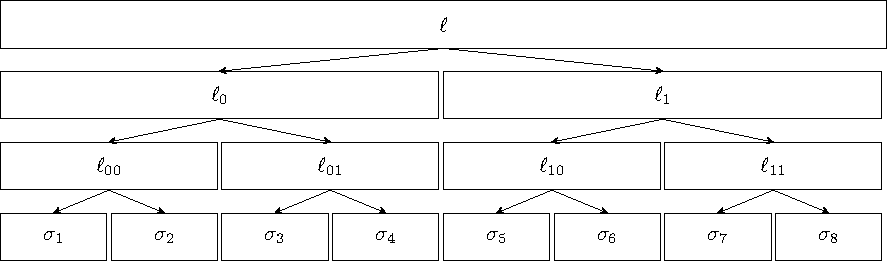
\includegraphics[width=\textwidth]{tikz/FalconTree}
\caption{A \falcon tree of height $3$}\label{fig:falcontree}
\end{figure}

The contents of a \falcon tree \tree are computed from the private key
elements $f$, $g$, $F$ and $G$ using the algorithm described in
\cref{sec:spec:keygen:ffldl} (see also \cref{alg:keygen}).

\subsection{Public key}

The \falcon public key \pk corresponding to the private key $\sk =
(f,g,F,G)$ is a polynomial $h \in \bZ_q[x]/(\phi)$ such that:
 \begin{equation}
  h = gf^{-1} \bmod (\phi,q).
 \end{equation}

\begin{code}
  type publicKey = Poly _n (Z q)
\end{code}

 \section{FFT and NTT} \label{sec:spec:fftntt}

\begin{code}
  // Helper functions for Complex Numbers
  CMul : (C, C) -> C
  CMul(x, y) = (x.0*y.0-x.1*y.1, x.0*y.1+x.1*y.0)

  CAdd : (C, C) -> C
  CAdd(x, y) = (x.0 + x.1, y.0 + y.1)

  CSub : (C, C) -> C
  CSub(x, y) = (x.0 - x.1, y.0 - y.1)

  CAddList : {n} (fin n) => [n]C -> C
  CAddList(l) = sums ! 0
    where sums = [zero] # [CAdd(el,sums') | el <- l
                                          | sums' <- sums
                          ]

  Conjugate : C -> C
  Conjugate((x, y)) = (x, -y)

  PolyConj : {k, n} (isPowerOfTwo k n) => Poly n C -> Poly n C
  PolyConj(f) = map Conjugate f

  dot : {n} (fin n) => FFT n -> FFT n -> FFT n
  dot f g = [CMul(fi,gi) | fi <- f | gi <- g]

  add : {n} (fin n) => FFT n -> FFT n -> FFT n
  add f g = [CAdd(fi,gi) | fi <- f | gi <- g]

  sub : {n} (fin n) => FFT n -> FFT n -> FFT n
  sub f g = [CSub(fi,gi) | fi <- f | gi <- g]

  one : {k, n} (isPowerOfTwo k n) => FFT n
  one = [(1.0,0.0) | i <- [0 .. (n-1)]]

  HadamardDivision : {n} (fin n) => FFT n -> FFT n -> FFT n
  HadamardDivision f g = dot f (map Cinv g)

  Cinv : C -> C
  Cinv((a,b)) = (a/.denominator, -(b/.denominator)) where
    denominator = a^^2 + b^^2
\end{code}
\begin{code}
  // Vector Operations
  dotVecVec : {m,n} (fin m, fin n) => [m](FFT n) -> [m](FFT n) -> (FFT n)
  dotVecVec fvec gvec = foldl add zero (zipWith dot fvec gvec)

  subVecVec : {m,n} (fin m, fin n) => [m](FFT n) -> [m](FFT n) -> [m](FFT n)
  subVecVec fvec gvec = [sub f g | f <- fvec | g <- gvec]

  addVecVec : {m,n} (fin m, fin n) => [m](FFT n) -> [m](FFT n) -> [m](FFT n)
  addVecVec fvec gvec = [add f g | f <- fvec | g <- gvec]

  dotVecMat : {m,l,n} (fin m, fin l, fin n) =>
    [m](FFT n) -> [m][l](FFT n) -> [l](FFT n)
  dotVecMat vector matrix = [dotVecVec vector v | v <- (transpose matrix)]

  NormalizePoly : {k, n} (isPowerOfTwo k n) =>
    (Float64, Poly n C) -> Poly n C
  NormalizePoly(_q, F) = dot F [Cinv(_q,0) | i <- [0 .. (n-1)]]
\end{code}

\begin{code}
  // Necessary casting functions
  IntToCmplx : ZZ -> C
  IntToCmplx(x) = ((fromInteger x),zero)

  CmplxToInt : C -> ZZ
  CmplxToInt(x) = roundToEven x.0

  CmplxToQ : C -> Q
  CmplxToQ(x) = fpToRational (x.0)

  IntPolyToCmplxPoly : {k, n} (isPowerOfTwo k n) => Poly n ZZ -> Poly n C
  IntPolyToCmplxPoly(f) = map IntToCmplx f

  CmplxPolyToIntPoly : {k, n} (isPowerOfTwo k n) => Poly n C -> Poly n ZZ
  CmplxPolyToIntPoly(f) = map CmplxToInt f

  CmplxPolyToQPoly : {k, n} (isPowerOfTwo k n) => Poly n C -> Poly n Q
  CmplxPolyToQPoly(f) = map CmplxToQ f
\end{code}
 % TODO: ternary case

 \paragraph{The \fft.} Let $f \in \bQ[x]/(\phi)$. We note $\Omega_\phi$ the set of complex roots of $\phi$. We suppose that $\phi$ is monic with distrinct roots over $\bC$, so that $\phi(x) = \prod\limits_{\zeta \in \Omega_\phi} (x - \zeta)$. We denote by $\fft_\phi(f)$ the fast Fourier transform of $f$ with respect to $\phi$:
 \begin{equation}
  \fft_\phi(f) = (f(\zeta))_{\zeta \in \Omega_\phi}
 \end{equation}
 When $\phi$ is clear from context, we simply note $\fft(f)$. We may also use the notation $\hat f$ to indicate that $\hat f$ is the \fft of $f$. $\fft_\phi$ is a ring isomorphism, and we note $\ifft_\phi$ its inverse. The multiplication in the \fft domain is denoted by $\fdot$. We extend the \fft and its inverse to matrices and vectors by component-wise application.

\begin{code}
  FFT : {k, n} (isPowerOfTwo k n) => Poly n C -> FFT n
  FFT(x)
    | k == 0 => x
    | k >  0 => resize(join([result0,result1])) where
        even = [x@(2*i  ) | i <- [0 .. (2^^(k-1)-1)]]
        odd =  [x@(2*i+1) | i <- [0 .. (2^^(k-1)-1)]]
        left = FFT`{k-1}(even)
        right = FFT`{k-1}(odd)
        X = join([left,right])
        result0 =
          [X@i + CMul(Omega_phi@(`n*i),(X@(i+`n/2))) | i <- [0 .. (n/2-1)]]
        result1 =
          [X@i - CMul(Omega_phi@(`n*i),(X@(i+`n/2))) | i <- [0 .. (n/2-1)]]

  invFFT  : {k, n} (isPowerOfTwo k n) => (FFT n) -> (Poly n C)
  invFFT(x) = FFT`{k}(x)

  PolyMulInC : {k, n} (isPowerOfTwo k n) =>
    ((Poly n C), (Poly n C)) -> (Poly n C)
  PolyMulInC(f, g) = invFFT`{k}(dot (FFT`{k} f) (FFT`{k} g))

  PolyDivInC : {k, n} (isPowerOfTwo k n) =>
    ((Poly n C), (Poly n C)) -> (Poly n C)
  PolyDivInC(f, g) = invFFT`{k}(HadamardDivision`{n} (FFT`{k} f) (FFT`{k} g))

  PolyMulInZ : {k, n} (isPowerOfTwo k n) =>
    ((Poly n ZZ), (Poly n ZZ)) -> (Poly n ZZ)
  PolyMulInZ(f, g) = CmplxPolyToIntPoly`{k}
    (PolyMulInC`{k}(IntPolyToCmplxPoly`{k} f, IntPolyToCmplxPoly`{k} g))

  // The result is in Poly n Q since we divide
  PolyDivInZ : {k, n} (isPowerOfTwo k n) =>
    ((Poly n ZZ), (Poly n ZZ)) -> (Poly n Q)
  PolyDivInZ(f, g) = CmplxPolyToQPoly`{k}
    (PolyDivInC`{k}(IntPolyToCmplxPoly`{k} f, IntPolyToCmplxPoly`{k} g))

  FFT' : {k, n} (isPowerOfTwo k n) => Poly n ZZ -> FFT n
  FFT'(x) = FFT`{k} (IntPolyToCmplxPoly`{k} x)

  invFFT' : {k, n} (isPowerOfTwo k n) => FFT n -> Poly n ZZ
  invFFT'(x) = CmplxPolyToIntPoly`{k}(invFFT`{k} x)

  FFT'' : {k, n} (isPowerOfTwo k n) => Poly n (Z q) -> FFT n
  FFT''(x) = FFT'`{k}(map fromZ x)
\end{code}

 Additions, subtractions, multiplications and divisions of polynomials
 modulo $\phi$ can be computed in FFT representations by simply
 performing them on each coordinate. In particular, this makes
 multiplications and divisions very efficient.

 For $\phi = x^n + 1$, the set of complex roots $\zeta$ of $\phi$ is:
 \begin{equation}\label{eq:phi}
 \Omega_\phi = \left\{\left. \exp\left(\frac{i (2k+1)\pi}{n}\right) \right| 0 \leq k < n \right\}
 \end{equation}
\begin{code}
  // We precompute all roots and store them in Omega_phi.
  // Check falcon_512.cry and falcon_1024.cry
\end{code}

 \paragraph{A note on implementing the \fft.} There exist several ways of implementing the \fft, which may yield slightly different results. For example, some implementations of the \fft scale our definition by a constant factor (\eg $1/\deg(\phi)$). Another differentiation point is the order of (the roots of) the \fft. Common orders are the increasing order (\ie the roots are sorted by their order on the unit circle, starting at $1$ and moving clockwise) or (variants of) the bit-reversal order. In the case of \falcon:
 \begin{itemize}
  \item The \fft is not scaled by a constant factor.
  \item There is no constraint on the order of the \fft, the choice is left to the implementer. However, the chosen order shall be consistent for all the algorithms using the \fft.
 \end{itemize}


 \paragraph{Representation of polynomials in algorithms.} The algorithms which specify \falcon heavily rely on the fast Fourier transform, and some of them explicitly require that the inputs and/or outputs are given in \fft representation. When the directive ``\algorithmicformat'' is present at the beginning of an algorithm, it specifies in which format (coefficient or \fft representation) the input/output polynomials shall be represented. When the directive ``\algorithmicformat'' is absent, no assumption on the format of the input/output polynomials is made.

\begin{code}
  type FFT degree = Poly degree C
\end{code}

 \paragraph{The NTT.} The NTT (Number Theoretic Transform) is the analog
 of the FFT in the field $\bZ_p$, where $p$ is a prime such that $p = 1
 \bmod 2n$. Under these
 conditions, $\phi$ has exactly $n$ roots $(\omega_i)$ over $\bZ_p$, and
 any polynomial $f \in \bZ_p[x]/(\phi)$ can be represented by the values
 $f(\omega_i)$. Conversion to and from NTT representation can be done
 efficiently in $O(n \log n)$ operations in $\bZ_p$. When in NTT
 representation, additions, subtractions, multiplications and divisions
 of polynomials (modulo $\phi$ and $p$) can be performed coordinate-wise
 in $\bZ_p$.

\begin{code}
  /* Recursive NTT */
  parameter
    r : Z q

  roots : [inf](Z q)
  roots = iterate ((*) (r * r)) 1

  NTT : {k, n} (isPowerOfTwo k n) => Poly n (Z q) -> Poly n (Z q)
  NTT a = ntt_r`{lg2 n} 0 a

  ntt_r : {n} (fin n) =>
    Integer -> [2 ^^ n](Z q) -> [2 ^^ n](Z q)
  ntt_r depth a
    | n == 0 => a
    | n > 0 => butterfly depth even odd
      where
        (lft, rht) = shuffle a
        even = ntt_r`{max 1 n - 1} (depth + 1) lft
        odd = ntt_r`{max 1 n - 1} (depth + 1) rht

  shuffle : {n, a} (fin n, n > 0) => [2 * n]a -> ([n]a, [n]a)
  shuffle a =
    ([ a @ (i * 2) | i <- [0 .. <n]], [ a @ (i * 2 + 1) | i <- [0 .. <n]])

  butterfly : {n} (fin n, n > 0) =>
    Integer -> [n](Z q) -> [n](Z q) -> [2 * n](Z q)
  butterfly depth even odd =
    lft # rht
    where
      j = 2 ^^ depth
      lft = [ even @ i + roots @ (i * j) * odd @ i | i <- [0 .. <n] ]
      rht = [ even @ i - roots @ (i * j) * odd @ i | i <- [0 .. <n] ]
\end{code}

\begin{code}
  /* INVERSE NTT */

  ivn : (Z q)
  ivn = recip (`_n : (Z q))

  ivr : (Z q)
  ivr = recip r

  ivroots : [inf](Z q)
  ivroots = iterate ((*) (ivr * ivr)) 1

  NTTInv : {k, n} (isPowerOfTwo k n) => Poly n (Z q) -> Poly n (Z q)
  NTTInv a =
    map ((*) ivn) (ivntt_r`{lg2 n} 0 a)

  ivntt_r : {n} (fin n) => Integer -> [2 ^^ n](Z q) -> [2 ^^ n](Z q)
  ivntt_r depth a
    | n == 0 => a
    | n > 0 => ivbutterfly depth even odd
      where
        (lft, rht) = shuffle a
        even = ivntt_r`{max 1 n - 1} (depth + 1) lft
        odd = ivntt_r`{max 1 n - 1} (depth + 1) rht

  ivbutterfly : {n} (fin n, n > 0) =>
    Integer -> [n](Z q) -> [n](Z q) -> [2 * n](Z q)
  ivbutterfly depth even odd =
    lft # rht
    where
      j = 2 ^^ depth
      lft = [ even @ i + ivroots @ (i * j) * odd @ i | i <- [0 .. <n] ]
      rht = [ even @ i - ivroots @ (i * j) * odd @ i | i <- [0 .. <n] ]
\end{code}

\begin{code}
  prodZq : {k, n} (isPowerOfTwo k n) =>
    Poly n (Z q) -> Poly n (Z q) -> Poly n (Z q)
  prodZq f g = NTTInv`{k}((NTT`{k} f) * (NTT`{k} g))

  ModInv : Z q -> Z q
  ModInv(f) =  1/. f
\end{code}

 % Care must be taken that the roots of $\phi$ in $\bZ_p$ are unrelated to
 % the roots of $\phi$ in $\bC$. %TPr: as noticed by Gregor, there actually is a group morphism mapping the first set to the other
 In \falcon, the NTT allows for faster
 implementations of public key operations (using $\bZ_q$) and key pair
 generation (with various medium-sized primes $p$). Private key
 operations, though, rely on the fast Fourier sampling, which uses the
 FFT, not the NTT.

 \section{Splitting and Merging} \label{sec:spec:splitmerge}

 In this section, we make explicit the chains of isomorphisms described in \cref{sec:spec:techoverview}, by presenting splitting (resp. merging) operators which allow to travel these chains from right to left (resp. left to right).

 Let $\phi, \phi'$ be cyclotomic polynomials such that $\phi(x) = \phi'(x^2)$ (for example, $\phi(x) = x^n + 1$ and $\phi'(x) = x^{n/2} + 1$). We define operators which are at the heart of our signing algorithm. Our algorithms require the ability to split an element of $\bQ[x]/(\phi)$ into two smaller elements of $\bQ[x]/(\phi')$. Conversely, we require the ability to merge two elements of $\bQ[x]/(\phi')$ into an element of $\bQ[x]/(\phi)$.


 \paragraph{The \splitfft operator.} Let $n$ be the degree of $\phi$, and $f = \sum_{i=0}^{n-1} a_i x^i$ be an arbitrary element of $\bQ[x]/(\phi)$, $f$ can be decomposed uniquely as $f(x) = f_0(x^2) + xf_1(x^2)$, with $f_0, f_1 \in \bQ[x]/(\phi')$. In coefficient representation, such a decomposition is straightforward to write:
 \begin{equation}\label{eq:split}
 f_0 = \sum\limits_{0 \leq i < n/2} a_{2i} x^i \text{\ \ \ and\ \ \ }f_1 = \sum\limits_{0 \leq i < n/2} a_{2i+1} x^i
 \end{equation}
 In \eqref{eq:split}, we simply split $f$ with respect to its even or odd coefficients. With this notation, we note:
 \begin{equation}\label{eq:splitdef}
 \polsplit(f) = (f_0,f_1).
 \end{equation}
 In \falcon, polynomials are repeatedly split, multiplied together, split again and so forth. To avoid switching back and forth between the coefficient and \fft representation, we always perform the split operation in the \fft representation. It is defined in \longsplitfft.


 \begin{algorithm}%[H]
 \caption{$\splitfft(\fft(f))$}\label{alg:splitfft}
  \begin{algorithmic}[1]
  \Require {$\fft(f) = (f(\zeta))_{\zeta}$ for some $f \in \bQ[x]/(\phi)$}
  \Ensure {$\fft(f_0)= (f_0(\zeta'))_{\zeta'}$ and $\fft(f_1)= (f_1(\zeta'))_{\zeta'}$ for some $f_0,f_1 \in \bQ[x]/(\phi')$}
  \Format{All polynomials are in \fft representation.}
  \For{$\zeta$ such that $\phi(\zeta) = 0$ and Im$(\zeta) > 0$}
  \Comment{See \cref{eq:phi} with $0 \leq k < n/2$}
  \State{$\zeta' \gets \zeta^2$}
  \State{$f_0(\zeta') \gets \frac{1}{2} \left[ f(\zeta) + f(-\zeta) \right]$}
  \State{$f_1(\zeta') \gets \frac{1}{2\zeta} \left[ f(\zeta) - f(-\zeta) \right]$}
  \EndFor
  \Return{$(\fft(f_0), \fft(f_1))$}
  \end{algorithmic}
 \end{algorithm}

 \splitfft is \polsplit realized in the \fft representation: for any $f, \fft(\polsplit(f)) = \splitfft(\fft(f))$. Readers familiar with the Fourier transform will recognize that \splitfft is a subroutine of the inverse fast Fourier transform, more precisely the part which from $\fft(f)$ computes two \fft's twice smaller.

\begin{code}
  splitfft : {k, n} (isPowerOfTwo k n, n > 1) =>
    (FFT n) -> (FFT (n/2), FFT (n/2))
  splitfft FFTf = (resize(FFTf0), resize(FFTf1)) where
    FFTf0 = [FFTf@(2*i  ) | i <- [0 .. (2^^(k-1)-1)]]
    FFTf1 = [FFTf@(2*i+1) | i <- [0 .. (2^^(k-1)-1)]]
\end{code}

 \paragraph{The \mergefft operator.} With the previous notations, we define the operator \polmerge as follows:
 \begin{equation}\label{eq:merge}
 \polmerge(f_0,f_1) = f_0(x^2) + xf_1(x^2) \in \bQ[x]/(\phi).
 \end{equation}
 Similarly to \polsplit, it is often relevant from an efficiently standpoint to perform \polmerge in the \fft representation. This is done in \longmergefft.

 \begin{algorithm}%[H]
 \caption{$\mergefft(f_0,f_1)$}\label{alg:mergefft}
  \begin{algorithmic}[1]
  \Require {$\fft(f_0) = (f_0(\zeta'))_{\zeta'}$ and $\fft(f_1) = (f_1(\zeta'))_{\zeta'}$ for some $f_0,f_1 \in \bQ[x]/(\phi')$}
  \Ensure {$\fft(f) = (f(\zeta))_{\zeta}$ for some $f \in \bQ[x]/(\phi)$}
  \Format{All polynomials are in \fft representation.}
  \For{$\zeta$ such that $\phi(\zeta) = 0$}
  \Comment{See \cref{eq:phi}}
  \State{$\zeta' \gets \zeta^2$}
  \State{$f(\zeta) \gets f_0(\zeta') + \zeta f_1(\zeta')$}
 %  \State{$f(-\zeta) \gets f_0(\zeta') - \zeta f_1(\zeta')$}
  \EndFor
  \Return{$\fft(f)$}
  \end{algorithmic}
 \end{algorithm}

\begin{code}
  mergefft : {k, n} (isPowerOfTwo k n, n>=2) =>
    (FFT (n/2), FFT (n/2)) -> (FFT n)
  mergefft (f0, f1) = resize FFTf where
    FFTf = join[[f0@i,f1@i] | i <- [0 .. (2^^(k-1)-1)]]
\end{code}

 It is immediate that \polsplit and \polmerge are inverses of each other, and equivalently \splitfft and \mergefft are inverses of each other. Just as for \splitfft, readers familiar with the Fourier transform can observe that \mergefft is a step of the fast Fourier transform: it is the reconstruction step which from two small \fft's computes a larger \fft.

\begin{code}
  FFTInvFFT : (FFT 4) -> Bit
  property FFTInvFFT f = mergefft`{2,4} (splitfft`{2,4} f) == f
\end{code}

 \paragraph{Relationship with the \fft.} There is no requirement on the order in which the values $f(\zeta)$ (resp. $f_0(\zeta')$, resp. $f_1(\zeta')$) are to be stored, and the choice of this order is left to the implementer. It is however recommended to use a unique order convention for the \fft, \ifft, \splitfft and \mergefft operators. Since the \fft and \ifft need to implemented anyway, this unique convention can be achieved \eg by implementing \splitfft as part of \ifft, and \mergefft as part of the \fft.

 \tprcomment{should we provide an example of \fft/\ifft algorithm?}

 The intricate relationships between the \polsplit and \polmerge operators, their counterparts in the \fft representation and the (inverse) fast Fourier transform are illustrated in the commutative diagram of \cref{fig:splitmerge}.

 \begin{figure}%[H]
 \centering
 \begin{tikzpicture}[]
 \matrix (m) [matrix of nodes,row sep=15mm,column sep = 25mm,draw=none]
 {
 $f\in \bQ[x]/(\phi)$ & $f_0,f_1 \in \bQ[x]/(\phi')$ \\
 $\hat f\in \fft(\bQ[x]/(\phi))$ & $\hat f_0, \hat f_1 \in \fft(\bQ[x]/(\phi'))$ \\
 };
 \draw[line] (m-1-1.259) -> (m-2-1.100) node[midway,left] {\fft};
 \draw[line] (m-1-2.259) -> (m-2-2.100) node[midway,left] {\fft};
 \draw[line] (m-2-1.80) -> (m-1-1.281) node[midway,right] {\ifft};
 \draw[line] (m-2-2.80) -> (m-1-2.281) node[midway,right] {\ifft};

 \draw[line] ($(m-1-1.east)+(0,.1)$) -> ($(m-1-2.west)+(0,.1)$) node[midway,above] {\polsplit~\eqref{eq:splitdef}};
 \draw[line] ($(m-2-1.east)+(0,.1)$) -> ($(m-2-2.west)+(0,.1)$) node[midway,above] {\splitfft};
 \draw[line] ($(m-1-2.west)-(0,.1)$) -> ($(m-1-1.east)-(0,.1)$) node[midway,below] {\polmerge~\eqref{eq:merge}};
 \draw[line] ($(m-2-2.west)-(0,.1)$) -> ($(m-2-1.east)-(0,.1)$) node[midway,below] {\mergefft};

 \end{tikzpicture}
 \caption{Relationship between \fft, \ifft, \polsplit, \polmerge, \splitfft and \mergefft}\label{fig:splitmerge}
 \end{figure}

 \subsection{Algebraic interpretation}\label{sec:spec:splitmerge:algebraic}

   The purpose of the splitting and merging operators that we defined is not only to represent an element of $\bQ[x]/(\phi)$ using two elements of $\bQ[x]/(\phi')$, but to do so in a manner compatible with ring operations. As an illustration, we consider the operation:
  \begin{equation}\label{eq:simpleproduct}
  a = b c
  \end{equation}
 where $a, b, c \in \bQ[x]/(\phi)$. For $f \in \bQ[x]/(\phi)$, we consider the associated endomorphism $\psi_f : z \in \bQ[x]/(\phi) \mapsto fz$. \eqref{eq:simpleproduct} can be rewritten as $a = \psi_c(b)$. By the $\polsplit$ isomorphism, $a$ and $b$ (resp. $\psi_c$) can also be considered as elements (resp. an endomorphism) of $(\bQ[x]/(\phi'))^2$. We can rewrite \eqref{eq:simpleproduct} as:
    \begin{equation}\label{eq:bisection}
   \onetwo{a_0}{a_1} = \onetwo{b_0}{b_1}  \twotwo{c_{0}}{c_{1}}{x c_{1}}{c_{0}}
    \end{equation}

  More formally, we have used the fact that splitting operators are isomorphisms between $\bQ[x]/(\phi)$ and $(\bQ[x]/(\phi'))^k$, which express elements of $\bQ[x]/(\phi)$ in the $(\bQ[x]/(\phi'))$-basis $\{1,x\}$ (hence ``breaking'' $a,b$ in vectors over a smaller field). Similarly, writing the transformation matrix of the endomorphism $\psi_c$ in the basis $\{1,x\}$ yields the $2\times 2$ matrix of \eqref{eq:bisection}.

 %\subsection{Relationship with the field norm}\label{sec:spec:splitmerge:fieldnorm} The splitting and merging operators allow to easily express the field norm for some specific cyclotomic fields. Let $\bL = \bQ[x]/(\phi), \bK = \bQ[x]/(\phi')$ and $f \in \bL$. Since by definition $\N_{\bL/\bK}(f) = \det_\bK(\psi_d)$, we can use \eqref{eq:bisection} to compute it explicitly. This yields:
 %\begin{itemize}
 % \item If $\phi'(x^2) = \phi(x)$, then $\N_{\bL/\bK}(f) = f_0^2 - x f_1^2$, where $(f_0, f_1) = \polsplit(f)$;
 %\end{itemize}
 %
 %For $f \in \bL$ with $\bL = \bQ[x]/(x^{2^\kappa} + 1)$, we also denote $\N(f) = f_0^2 - x f_1^2 = \N_{\bL/\bK}(f)$, where $\bK$ is the largest strict subfield of $\bL$ (see \eqref{eq:binarytower}). For the values of $\phi$ considered in this document, this allows to define $\N(f)$ in an unambiguous way.

 %\tprcomment{I simplified everything related to the field norm, it was too verbose}

 \paragraph{Relationship with the field norm.} The field norm (or relative norm) $\N_{\bL/\bK}$ maps elements of a larger field $\bL$ onto a subfield $\bK$. It is an important notion in field theory, but in this document, we only need to define it for a simple, particular case. Let $n = 2^\kappa$ a power of two, $\bL = \bQ[x]/(x^{n} + 1)$ and $\bK = \bQ[x]/(x^{n/2} + 1)$. We define the field norm $\N_{\bL/\bK}$ as follows:
 \begin{equation}\label{eq:fieldnorm}
 \begin{array}{llllc}
 \N_{\bL/\bK} & : & \bL & \rightarrow & \bK \\
 & & f & \mapsto & f_0^2 - x f_1^2
 \end{array}
 \end{equation}
 where $(f_0,f_1) = \polsplit(f) \in \bK^2$, see \eqref{eq:split} and \eqref{eq:splitdef} for explicit formulae. When $\bL$ and $\bK$ are clear from context, we simply note $\N(f) = \N_{\bL/\bK}(f)$. An equivalent formulation for $\N_{\bL/\bK}$ is:
 \begin{equation}\label{eq:fieldnormmul}
 \N_{\bL/\bK} (f) = f(x) \cdot f(-x)
 \end{equation}
 Both \eqref{eq:fieldnorm} and \eqref{eq:fieldnormmul} are valid formulae for $\N_{\bL/\bK}(f)$, but \eqref{eq:fieldnorm} is more suited to the coefficient representation, and \eqref{eq:fieldnormmul} is more suited to the NTT representation.

\begin{code}
  // N is only used on integer polynomials in NTRUSolve
  // so we set its type accordingly.
  N : {k, n} (isPowerOfTwo k n, k > 0) =>
    (Poly n ZZ) -> (Poly (2^^(k-1)) ZZ)
  N(f) = f0sq + minusxf1sq where
    (_f0, _f1) = splitfft`{k} (IntPolyToCmplxPoly`{k} f) // split*fft*
    f0 = CmplxPolyToIntPoly`{k-1} (resize _f0)
    f1 = CmplxPolyToIntPoly`{k-1} (resize _f1)
    f0sq = PolyMulInZ`{k-1}(resize f0, resize f0)
    f1sq = PolyMulInZ`{k-1}(resize f1, resize f1)
    minusxf1sq = [0] # [-(f1sq@i) | i <- [1..<(2^^(k-1))]]
\end{code}

 \section{Hashing} \label{sec:spec:hash}

As for any hash-and-sign signature scheme, the first step to sign a message or verify a signature consists of hashing the message. In our case, the message needs to be hashed into a polynomial in $\bZ_q[x]/(\phi)$. An approved extendable-output hash function (XOF), as specified in FIPS 202~\cite{FIPS}, shall be used during this procedure.

This XOF shall have a security level at least equal to the security level targeted by our signature scheme. In addition, we should be able to start hashing a message without knowing the security level at which it will be signed. For these reasons, we use a unique XOF for all security levels: \shake.
\begin{itemize}
 \item \shakeinit() denotes the initialization of a \shake hashing context;
 \item \shakeinject(\shakectx, \str) denotes the injection of the data \str in the hashing context \shakectx;
 \item \shakeextract(\shakectx, $b$) denotes extraction from a hashing context \shakectx of $b$ bits of pseudorandomness.
\end{itemize}

\longhashtopoint defines the hashing process used in \falcon. It is defined for any $q \leq 2^{16}$. In \falcon, big-endian convention is used to interpret a chunk of $b$
bits, extracted from a \shake instance, into an integer in the $0$ to
$2^b-1$ range (the first of the $b$ bits has numerical weight $2^{b-1}$,
the last has weight $1$).

\begin{algorithm}[htb]
\caption{$\hashtopoint(\str, q, n)$}\label{alg:hashtopoint}
\begin{algorithmic}[1]
\Require{A string \str, a modulus $q \leq 2^{16}$, a degree $n \in \bN^\star$}
\Ensure{An polynomial $c = \sum_{i=0}^{n-1} c_i x^i $ in $\bZ_q[x]$}
\State{$k \gets \lfloor 2^{16}/q \rfloor$}
\State{$\shakectx \gets \shakeinit()$}
\State{$\shakeinject(\shakectx, \str)$}
\State{$i \gets 0$}
\While{$i < n$}
\State{$t \gets \shakeextract(\shakectx, 16)$}\label{step:extract}
\If{$t < k q$} \label{alg:hashtopoint:cmp}\label{step:check}
\State{$c_i \gets t \bmod q$} \label{alg:hashtopoint:mod}
\State{$i \gets i+1$}
\EndIf
\EndWhile
\Return{$c$}
\end{algorithmic}
\end{algorithm}

\begin{code}
  import Primitive::Keyless::Hash::SHAKE::SHAKE256
  HashToPoint : {q', k, n, len}
    (q' <= 2^^16, q' >= 1, isPowerOfTwo k n, fin len) =>
    [len] -> Poly n (Z q')
  HashToPoint str = take`{n} (HashToPointInf`{q'} (shake256 str))

  HashToPointInf : {q'} (q' <= 2^^16, q' >= 1) =>
    [inf] -> Poly inf (Z q')
  HashToPointInf hash =
    if t < toInteger(k*`q') then
      [ci] # HashToPointInf tailH
    else
      HashToPointInf tailH
    where
      t = toInteger(take`{16} hash)
      tailH = drop`{16} hash
      ci = fromInteger(toInteger(t%`q))
      k = 2^^16 / `q
\end{code}

\paragraph{Possible variants.}
\begin{itemize}

\item If $q > 2^{16}$, then larger chunks can be extracted from \shake
at each step.

\item \hashtopoint may be difficult to efficiently
implement in a constant-time way; constant-timeness may be a desirable
feature if the signed data is also secret.

A variant which is easier to
implement with constant-time code extracts $64$ bits instead of $16$ at
step~\ref{step:extract}, and omits the conditional check of
step~\ref{step:check}. While the omission of the check means that some
outputs are slightly more probable than others, a
Rényi argument~\cite{AC:BLLSS15,AC:Prest17} allows to claim that this variant is
secure for the parameters set by NIST~\cite{NIST}.

\end{itemize}

Of course, any variant deviating from the procedure expressed in
\cref{alg:hashtopoint} implies that the same message will hash
to a different value, which breaks interoperability.

% Algorithm~\ref{alg:hashtopoint} can be used to efficiently achieve this \hashtopoint operation. It is not constant-time but, for most applications, variable-time generation of the public parameter $c$ is not a problem. It is defined for $q \leq 2^{16}$ but can be easily adapted for arbitrary large $q$. As described in \cite{https://eprint.iacr.org/2016/467.pdf}, step~\ref{alg:hashtopoint:cmp}-\ref{alg:hashtopoint:mod} execute a rejection on the \shake output considered as an array of 16-bit, unsigned, little-endian integers. Each of those integers is used as a coefficient of $c$, after having been reduced modulo $q$, if it is smaller than $\lfloor 2^{16}/q \rfloor q$ and rejected otherwise.
%
% Note that, when timing leak of public information can be a problem, one can use the alternative approach described in \cite{USENIX:ADPS16} to parse the \shake output, which is more slower and incompatible with the straightforward approach described above, but does not leak any timing information about $c$.
%
% Todo: describe this constant-time approach?

% !TeX root = ../falcon.tex

\section{Key Pair Generation} \label{sec:spec:keygen}


\subsection{Overview}\label{sec:spec:keygen:overview}

The key pair generation can be decomposed in two clearly separate parts.
\begin{itemize}
 \item \emph{Solving the NTRU equation.} The first step of the key pair generation consists of computing polynomials $f, g, F, G \in \bZ[x]/(\phi)$ which verify \eqref{eq:ntru} -- the NTRU equation.
 Generating $f$ and $g$ is easy; the hard part is to efficiently compute polynomials $F,G$ such that \eqref{eq:ntru} is verified.

 To do this, we propose a novel method that exploits the tower-of-rings structure highlighted in \eqref{eq:binarytower}.
 We use the field norm $\N$ to map the NTRU equation onto a smaller ring $\bZ[x]/(\phi')$ of the tower of rings, all the way down to $\bZ$. We then solve the equation in $\bZ$ -- using an extended gcd -- and use properties of the norm to lift the solutions $(F,G)$ back to the original ring $\bZ[x]/(\phi)$.

 Implementers should be mindful that this step does \textit{not} perform modular reduction modulo $q$, which leads us to handle polynomials with large coefficients (a few thousands of bits per coefficient in the lowest levels of the recursion). See \cref{sec:spec:keygen:ntrugen} for a formal specification of this step, and \cite{PKC:PorPre19} for an in-depth analysis.

 \item \emph{Computing a \falcon tree.} Once suitable polynomials $f,g,F,G$ are generated, the second part of the key generation consists of preprocessing them into an adequate format: by adequate we mean that this format should be reasonably compact and allow fast signature generation on-the-go.

 \falcon trees are precisely this adequate format. To compute a \falcon tree, we compute the $\LDLs$ decomposition $\matG = \matL \matD \adj \matL$ of the matrix $\matG = \matB \adj \matB$, where
 \begin{equation}
 \matB = \twotwo{g}{-f}{G}{-F},
 \end{equation}
 which is equivalent to computing the Gram-Schmidt orthogonalization $\matB = \matL \times \tilde \matB$. If we were using Klein's well-known sampler (or a variant thereof) as a trapdoor sampler, knowing $\matL$ would be sufficient but a bit unsatisfactory as we would not exploit the tower-of-rings structure of $\bQ[x]/(\phi)$.

 So instead of stopping there, we store $\matL$ (or rather $L_{10}$, its bottom-left and only non-trivial term) in the root of a tree, use the splitting operators defined in \cref{sec:spec:splitmerge} to ``break'' the diagonal elements $D_{ii}$ of $\matD$ into matrices $\matG_i$ over smaller rings $\bQ[x]/(\phi')$, at which point we create subtrees for each matrix $\matG_i$ and recursively start over the process of $\LDLs$ decomposition and splitting.

 The recursion continues until the matrix $\matG$ has its coefficients in $\bQ$, which correspond to the bottom of the recursion tree. How this is done is specified in \cref{sec:spec:keygen:ffldl}.

 The main technicality of this part is that it exploits the tower-of-rings structure of $\bQ[x]/(\phi)$ by breaking its elements onto smaller rings. In addition, intermediate results are stored in a tree, which requires precise bookkeeping as elements of different tree levels do not live in the same field. Finally, for performance reasons, the step is realized completely in the \fft domain.
\end{itemize}

Once these two steps are done, the rest of the key pair generation is straightforward. A final step normalizes the leaves of the LDL tree to turn it into a \falcon tree. The result is wrapped in a private key \sk and the corresponding public key \pk is $h = g f^{-1} \bmod q$.


A formal description is given in algorithms \ref{alg:keygen} to \ref{alg:ffldl}, the main algorithm being the procedure \longkeygen. The general architecture of the key pair generation is also illustrated in \cref{fig:keygen}.

\begin{figure}[t]
\centering
\begin{tikzpicture}[every node/.style={draw=black}]
\matrix (m) [matrix of nodes,row sep=7mm,column sep = 1.5cm,draw=none]
{
& \keygen & \\
\ntrugen &  & \ffldl \\
\ntrusolve & & \ldlalgo \\
};
\draw[line] (m-1-2) -> (m-2-1);
\draw[line] (m-1-2) -> (m-2-3);
\draw[line] (m-1-2) -> (m-2-3);
\draw[line] (m-2-1) -> (m-3-1);
\draw[line] (m-2-3) -> (m-3-3);
\end{tikzpicture}
\caption{Flowchart of the key generation}\label{fig:keygen}
\end{figure}



 \begin{algorithm}[!htp]
  \caption{$\keygen(\phi, q)$}\label{alg:keygen}
 \begin{algorithmic}[1]
  \Require{A monic polynomial $\phi \in \bZ[x]$, a modulus $q$}
  \Ensure{A secret key $\sk$, a public key $\pk$}
  \State{$f,g,F,G \gets \ntrugen(\phi, q)$}\label{alg:keygen:ntru}\Comment{Solving the NTRU equation}
  \State{$\matB \gets \twotwo{g}{-f}{G}{-F}$}\label{alg:keygen:bgnhatb}
  \State{$\hat \matB \gets \fft(\matB)$} \Comment{Compute the FFT for each of the 4 components $\{g, -f, G, -F\}$}
  \State{$\matG \gets \hat\matB \times \adj{\hat\matB}$}\label{alg:keygen:endhatb}
  \State{$\tree \gets \ffldl(\matG)$}\label{alg:keygen:bgnftree}\Comment{Computing the $\LDLs$ tree}
%  \State{$\sigma \gets 1.55 \sqrt{q}$}
  \For{each leaf \leaf of \tree}\label{normal:start}\Comment{Normalization step}
  \State{$\leaf.\data \gets \sigma / \sqrt{\leaf.\data}$}\label{normal:end}
  \EndFor
  \State{$\sk \gets (\hat\matB, \tree)$}
  \State{$h \gets gf^{-1} \bmod q$}\label{alg:keygen:pk}
  \State{$\pk \gets h$}
  \Return{$\sk, \pk$}
  \end{algorithmic}
 \end{algorithm}

\begin{code}
  // phi and q are fixed so we do not parameterize this algorithm
  // f and g cannot be sampled in Cryptol so we take them as input
  Keygen : (Poly _n ZZ, Poly _n ZZ) -> (privateKey, publicKey)
  Keygen (f', g') = (sk, pk) where
    (f, g, F, G) = NTRUGen(f', g')
    B = [[map IntToCmplx g,map IntToCmplx (-f)],
         [map IntToCmplx G,map IntToCmplx (-F)]]
    Bhat = [[FFT'`{_k}(g),FFT'`{_k}(-f)],
            [FFT'`{_k}(G),FFT'`{_k}(-F)]]
    GG = B * Bhat
    T = ffLDLstar`{_k}(GG)
    leaves = get_leaves`{_k} T
    new_leaves = [(sigma/.r_leaf,0) | (r_leaf, _) <- leaves]
    T' = set_leaves`{_k}(T, new_leaves)
    sk = ([[f, g], [F, G]], Bhat, T')
    h = NTTInv`{_k}(NTT`{_k}(map fromInteger g)*
        (map ModInv (NTT`{_k}(map fromInteger f)))) // can be improved
    pk = h
\end{code}
% \pagebreak

\subsection{Generating the polynomials \texorpdfstring{$f,g,F,G$}{f, g, F, G}.}\label{sec:spec:keygen:ntrugen}

The first step of the key pair generation generates suitable polynomials $f,g,F,G$ verifying \eqref{eq:ntru}. This is specified in \longntrugen. We provide a general explanation of \ntrugen:
\begin{enumerate}
 \item First, the polynomials $f,g$ are generated randomly. A few conditions over $f,g$ are checked to ensure they are suitable for our purposes (\cref{step:ntt} to \cref{step:endgenfg}). It particular:
 \begin{enumerate}
  \item Line~\ref{step:ntt} ensures a public key $h$ can be computed from $f,g$. This is true if and only if $f$ is invertible $\bmod\ q$, which is true if and only if $\ntt(f)$ contains no coefficient set to $0$.
  \item The polynomials $f,g,F,G$ must allow to generate short signatures. This is true if:
  \begin{equation}
  \gamma~=~\max \left\{ \norm{(g,-f)},  \norm{\left(\frac{q\adj f}{\ffgg},\frac{q\adj g}{\ffgg}\right)} \right\} \leq 1.17\sqrt{q}.
  \end{equation}
  We recall that the norm $\|\cdot\|$ is easily computed by using \eqref{eq:norm} with either \eqref{eq:innerfft} or \eqref{eq:innercoef}, depending on the representation (FFT or coefficient).
 \end{enumerate}
 \item Second, short polynomials $F,G$ are computed such that $f,g,F,G$ verify \eqref{eq:ntru}. This is done by the procedure \longntrusolve.
 \end{enumerate}

\begin{algorithm}%[!htp]
  \caption{$\ntrugen(\phi, q)$ \hfill}\label{alg:ntrugen}
 \begin{algorithmic}[1]
  \Require{A monic polynomial $\phi \in \bZ[x]$ of degree $n$, a modulus $q$}
  \Ensure{Polynomials $f,g,F,G$}
%   \Format{The polynomials $\phi, f,g,F,G$ are in coefficient representation.}
  \State{$\sigmafg \gets  1.17 \sqrt{q/2n}$}\label{step:genfg}\Comment{$\sigmafg$ is chosen so that $\bE[\|(f,g)\|] = 1.17 \sqrt{q}$}
  \For{$i$ from $0$ to $n-1$}
  \State{$f_i \gets D_{\bZ,\sigmafg,0}$}\label{line:sigmafg} \Comment{See also \eqref{eq:sigmastar}}
  \State{$g_i \gets D_{\bZ,\sigmafg,0}$}
  \EndFor
  \State{$f \gets \sum_i f_i x^i$}\Comment{$f \in \bZ[x]/(\phi)$}\label{line:fi}
  \State{$g \gets \sum_i g_i x^i$}\Comment{$g \in \bZ[x]/(\phi)$}\label{line:gi}
  \If{$\ntt(f)$ contains $0$ as a coefficient}\label{step:ntt} \Comment{Check that $f$ is invertible $\bmod\ q$}
  \Restart
  \EndIf
  \State{$\gamma \gets \max \left\{ \norm{(g,-f)},  \norm{\left(\frac{q\adj f}{\ffgg},\frac{q\adj g}{\ffgg}\right)} \right\}$}\label{line:gamma}
  \Comment{Using \eqref{eq:norm} with \eqref{eq:innerfft} or \eqref{eq:innercoef}}
  \If{$\gamma > 1.17\sqrt{q}$}
  \Comment{Check that $\gamma = \gsnorm{\matB}$ is short}
  \Restart
  \EndIf\label{step:endgenfg}
% New NTRUSolve
  \State{$F, G \gets \ntrusolve_{n,q}(f, g)$} \Comment{Computing $F, G$ such that $fG - gF = q \bmod \phi$}
  \If{$(F,G) = \bot$}\label{line:botntrusolve}
  \Restart\label{line:botntrusolverestart}
  \EndIf
  \Return{$f,g,F,G$}
  \end{algorithmic}
\end{algorithm}

\begin{code}
  // phi and q are fixed so we do not parameterize this algorithm
  // f and g cannot be sampled in Cryptol so we take them as input
  // We assume they pass conditions in lines 7 and 10
  NTRUGen : (Poly _n ZZ, Poly _n ZZ) ->
    (Poly _n ZZ, Poly _n ZZ, Poly _n ZZ, Poly _n ZZ)
  NTRUGen(f, g) = (f, g, F, G) where
    (F, G) = NTRUSolve`{_k}(f, g)
\end{code}

\newcommand{\sigmastar}{{\sigma^*}}
One way to sample $z \gets D_{\sigmafg}$ (\cref{line:fi,line:gi}) is to perform:
\begin{equation}\label{eq:sigmastar}
z = \sum_{i = 1}^{4096/n} z_i, \quad \text{where} \begin{cases}
z_i \gets \samplerz(0, \sigmastar),\\
\sigmastar = 1.17 \cdot \sqrt\frac{q}{8192} \approx 1.43300980528773
\end{cases}
\end{equation}
This exploits the fact the sum of $k$ Gaussians of standard deviation $\sigmastar$ is a Gaussian of standard deviation $\sigmastar \sqrt{k}$. Here $\sigmastar$ is chosen so that $\sigmastar \leq \sigmax$, see \cref{sec:spec:sign:integers}. Note that the reference code currently implements a similar idea, but with a $\sigmastar > \sigmax$ for which we sample using a precomputed table.

 \subsubsection{Solving the NTRU equation \eqref{eq:ntru}}

 We now explain how to solve \eqref{eq:ntru}. As mentioned in \cref{sec:spec:keygen:overview}, we repeatedly use the field norm $\N$ to map $f,g$ to a smaller ring $\bZ[x]/(x^{n/2}+1)$, until we reach the ring $\bZ$. Solving \eqref{eq:ntru} then amounts to computing an extended GCD over $\bZ$, which is simple. We then use the multiplicative properties of the field norm to repeatedly lift the solutions up to $\bZ[x]/(x^{n}+1)$, at which point we have solved \eqref{eq:ntru}.

% \todo{Fix algorithm}

% \tprcomment{I changed lines 11 and 12 of \ntrusolve}

  \begin{algorithm}[!htp]
  \caption{$\ntrusolve_{n,q}(f, g)$\hfill}\label{alg:ntrusolve}
 \begin{algorithmic}[1]
  \Require{$f, g \in \bZ[x]/(x^n+1)$ with $n$ a power of two}
  \Ensure{Polynomials $F,G$ such that \eqref{eq:ntru} is verified}

  \If{$n=1$}
  \State{Compute $u,v \in \bZ$ such that $u f - v g = \gcd(f, g)$}\Comment{Using the extended GCD}
  \If{$\gcd(f, g) \neq 1$}\label{line:botgcd}
  \State{abort and return $\bot$}\label{line:botgcd2}
  \EndIf
  \State{$(F,G) \gets (vq, uq)$}
  \Return{$(F,G)$}
  \Else
  \State{$f' \gets \N(f)$}\Comment{$f', g', F', G' \in \bZ[x]/(x^{n/2}+1)$}
  \State{$g' \gets \N(g)$}\Comment{$\N$ as defined in either \eqref{eq:fieldnorm} or \eqref{eq:fieldnormmul}}
  \State{$(F',G') \gets \ntrusolve_{n/2,q}(f', g')$}\Comment{Recursive call}

  \State{$F \gets F'(x^2) g(-x)$}\label{line:g} \Comment{$F, G \in \bZ[x]/(x^{n}+1)$}
  \State{$G \gets G'(x^2) f(-x)$}\label{line:f}
  \State{$\reduce(f,g,F,G)$}\Comment{$(F,G)$ is reduced with respect to $(f,g)$}
  \EndIf
  \Return{$(F,G)$}
  \end{algorithmic}
 \end{algorithm}

\begin{code}
  xSquared : {k, n} (isPowerOfTwo k n) => (Poly n ZZ) -> (Poly (2^^(k+1)) ZZ)
  xSquared(F) = resize (join[[c,0] | c <- F])

  minusx : {k, n} (isPowerOfTwo k n) => (Poly n ZZ) -> (Poly n ZZ)
  minusx(g) = resize (join[ [g@i, -(g@(i+1))] | i <- [0, 2 .. (n-1)]])

  eGCD : (ZZ, ZZ) -> (ZZ, ZZ, ZZ)
  eGCD(a, b) =
    if a == 0
    then (b, 0, 1)
    else (g, t - (b / a) * s, s) where
      (g, s, t) = eGCD((b%a), a)

  NTRUSolve : {k, n} (isPowerOfTwo k n) =>
    (Poly n ZZ, Poly n ZZ) -> (Poly n ZZ, Poly n ZZ)
  NTRUSolve(f, g)
    | k == 0 => ([F], [G]) where
        (gcd, u, v) = eGCD(f@0, g@0)
        (F, G) = (u*`q, v*`q)
    | k >  0 => (_F, _G) where
        f' = N`{k}(f)
        g' = N`{k}(g)
        (F', G') = NTRUSolve`{k-1}(f',g')
        F = PolyMulInZ`{k}(xSquared`{k-1}(F'), minusx`{k}(g))
        G = PolyMulInZ`{k}(xSquared`{k-1}(G'), minusx`{k}(f))
        (_F, _G) = Reduce`{k}(f,g,F,G)
\end{code}

 \ntrusolve uses \longreduce as a subroutine to reduce the size of the solutions $F,G$.
 The principle of \reduce is a simple generalization of textbook vectors' reduction. Given vectors $\vecu, \vecv \in \bZ^k$, reducing $\vecu$ with respect to $\vecv$ is done by simply performing $\vecu \gets \vecu - \left\lfloor \frac{ \inner{\vecu}{\vecv} }{ \inner{\vecv}{\vecv} } \right\rceil \vecv$. \reduce does the same by replacing $\bZ^k$ by $(\bZ[x]/(\phi))^2$, $\vecu$ by $(F,G)$ and $\vecv$ by $ (f,g)$. A detailed explanation of the mathematical and algorithmic principles underlying \ntrusolve can be found in~\cite{PKC:PorPre19}.

  \begin{algorithm}[!htp]
  \caption{$\reduce(f,g,F,G)$}\label{alg:reduce}
 \begin{algorithmic}[1]
  \Require{Polynomials $f,g,F,G \in \bZ[x]/(\phi)$}
  \Ensure{$(F,G)$ is reduced with respect to $(f,g)$}

  \Do
  \State{$k \gets \left \lfloor \frac{F\adj f + G\adj g}{\ffgg}\right\rceil$}
  \Comment{$\frac{F\adj f + G\adj g}{\ffgg} \in \bQ[x]/(\phi)$ and $k \in \bZ[x]/(\phi)$}
  \State{$F \gets F - k f$}
  \State{$G \gets G - k g$}
  \doWhile{$k \neq 0$}
  \Comment{Multiple iterations may be needed, e.g. if $k$ is computed in small precision.}
  \end{algorithmic}
 \end{algorithm}

\begin{code}
  Reduce : {k, n} (isPowerOfTwo k n) =>
    (Poly n ZZ, Poly n ZZ, Poly n ZZ, Poly n ZZ) -> (Poly n ZZ, Poly n ZZ)
  Reduce(f,g,F,G) = (F', G') where
    reduce_body(k_, F_, G_) = (k_', F_', G_') where
      numerator =
	    PolyMulInZ`{k}(F_, star`{n}(f)) + PolyMulInZ`{k}(G_, star`{n}(g))
      denominator =
	    PolyMulInZ`{k}(f, star`{n}(f)) + PolyMulInZ`{k}(g, star`{n}(g))
      k_' = map roundToEven (PolyDivInZ`{k}(numerator, denominator))
      F_' = F - PolyMulInZ`{k}(k_,f)
      G_' = G - PolyMulInZ`{k}(k_, g)
    k_not_zero(k_, F_, G_) = k_ != zero
    (_, F', G') = dowhile k_not_zero reduce_body zero
\end{code}

\clearpage

\subsection{Computing a \falcon Tree} \label{sec:spec:keygen:ffldl}

 The second step of the key generation consists of preprocessing the polynomials $f,g,F,G$ into an adequate secret key format. The secret key is of the form $\sk = (\hat\matB, \tree)$, where:
 \begin{itemize}
 \item $\hat\matB = \twotwo{\fft(g)}{-\fft(f)}{\fft(G)}{-\fft(F)}$
 \item \tree is a \falcon tree computed in two steps:
 \begin{enumerate}
 \item First, a tree \tree is computed from $\matG \gets \hat \matB \times \adj{\hat\matB}$, called an \emph{LDL tree}. This is specified in \longffldl. At this point, \tree is a \falcon tree but it is not normalized.
 \item Second, $\tree$ is normalized with respect to a standard deviation $\sigma$. It is described in steps \ref{normal:start}-\ref{normal:end} of \longkeygen.
 \end{enumerate}
 For efficiency reasons, polynomials manipulated in \longldlalgo and \longffldl always remain in \fft representation.
 \end{itemize}

 At a high level, the method for computing the LDL tree at step 1 (before normalization) is simple:
 \begin{enumerate}
  \item We compute the LDL decomposition of $\matG$: we write $\matG = \matL \times \matD \times \adj{\matL} $, with $\matL$ a lower triangular matrix with $1$'s on the diagonal and $\matD$ a diagonal matrix. See \longldlalgo.

  We store $\matL$ in \tree.\data, which is the value of the root of \tree. Since $\matL$ is of the form $\matL = \twotwo{1}{\ \ \ 0\ \ \ }{L_{10}}{1}$, we only need to store $L_{10} \in \bQ[x]/(\phi)$.

  \item We then use the splitting operator to ``break'' each diagonal element of $\matD$ into a matrix of smaller elements. More precisely, for a diagonal element $d \in \bQ[x]/(x^n + 1)$, we consider the associated endomorphism $\psi_d : z \in \bQ[x]/(x^n + 1) \mapsto dz$ and write its transformation matrix over the smaller ring $\bQ[x]/(x^{n/2} + 1)$. Following the argument of \cref{sec:spec:splitmerge:algebraic}, the transformation matrix of $\psi_d$ can be written as
   \begin{equation}\label{eq:matsplit1}
    \twotwo{d_{0}}{d_{1}}{x d_{1}}{d_{0}} \left( =  \twotwo{d_{0}}{d_{1}}{\adj d_{1}}{d_{0}} \right)\footnote{The equality in parentheses is true if and only if d is self-adjoint, \ie $\adj d = d$. This is the case in \longffldl.}.
   \end{equation}

  For each diagonal element broken into a self-adjoint matrix $\matG_i$ over a smaller ring, we recursively compute its LDL tree as in step 1 and store the result in the left or right child of \tree (which we denote \tree.\lchild and \tree.\rchild respectively).

  We continue the recursion until we end up with coefficients in the ring $\bQ$.

 \end{enumerate}

 An implementation of this ``LDL tree'' strategy is given in \longffldl. Note that in \falcon, the input of \ffldl is always a matrix of dimension $2 \times 2$, which greatly simplifies the implementation of its subroutine \longldlalgo.

% \tprcomment{Should we simplify the description of \ldlalgo?}

% \tprcomment{Corrected a typo}
% \begin{algorithm}[!htp]
% \caption{$\ldlalgo(\matG)$}\label{alg:ldlalgo}
% \begin{algorithmic}[1]
% \Require {A full-rank autoadjoint matrix $\matG = (G_{ij}) \in \fft(\bQ[x]/(\phi))^{\ell \times \ell }$}
% \Ensure {The \LDLs decomposition $\matG = \L \matD \adj\L$ over $\fft(\bQ[x]/(\phi))$}
%  \Format{All polynomials are in \fft representation.}
% \State{$\L, \matD \gets \matzero^{\ \ell \times \ell }$}
% \For{$i$ from $0$ to $(\ell - 1)$}
% \State{$\l_{ii} \gets 1$}
% \For{$j$ from $0$ to $(i-1)$}
% \State {$\l_{ij} \gets \frac{1}{D_{j}} \left( G_{ij} -  \sum_{k<j} \l_{ik} \fdot  \adj \l_{jk} \fdot D_k \right)$}
% \EndFor
% \State {$D_{i} \gets G_{ii} - \sum_{j<i} \l_{ij} \fdot \adj \l_{ij} \fdot D_j$}
% \EndFor
% \Return{$(\L, \matD )$} \Comment{$\matL = \twotwo{1}{0}{L_{10}}{1}, \matD = \twotwo{D_{00}}{0}{0}{D_{11}}$}
% \end{algorithmic}
% \end{algorithm}

%\tprcomment{Attempt at simplified version}

\begin{algorithm}[!htb]
	\caption{$\ldlalgo(\matG)$}\label{alg:ldlalgo}
	\begin{algorithmic}[1]
		\Require {A full-rank self-adjoint matrix $\matG = (G_{ij}) \in \fft(\bQ[x]/(\phi))^{2 \times 2}$}
		\Ensure {The \LDLs decomposition $\matG = \L \matD \adj\L$ over $\fft(\bQ[x]/(\phi))$}
		\Format{All polynomials are in \fft representation.}
		\State{$D_{00} \gets G_{00}$}
		\State{$\l_{10} \gets G_{10} / G_{00} $}
		\State{$D_{11} \gets G_{11} - \l_{10} \fdot \adj \l_{10} \fdot G_{00}$}
		\State{$\matL \gets \twotwo{1}{0}{L_{10}}{1}, \matD \gets \twotwo{D_{00}}{0}{0}{D_{11}}$}
		\Return{$(\L, \matD )$}
	\end{algorithmic}
\end{algorithm}

\begin{code}
  LDLstar : {k, n} (isPowerOfTwo k n) =>
    [2][2](FFT n) -> (([2][2](FFT n)), ([2][2](FFT n)))
  LDLstar(G) = (L, D) where
    D00 = G@0@0
    L10 = HadamardDivision (G@1@0) (G@0@0): FFT n
    D11 = G@1@1 - dot L10 (dot (PolyConj`{k}(L10)) (G@0@0))
    L = [[one`{k}, zero],[L10, one`{k}]]
    D = [[D00, zero],[zero, D11]]
\end{code}

 \begin{algorithm}[!htb]
 \caption{$\ffldl(\matG)$\hfill}\label{alg:ffldl}
 \begin{algorithmic}[1]
 \Require {A full-rank Gram matrix $\matG \in \fft\left(\bQ[x]/(x^n+1)\right)^{2\times 2}$}
 \Ensure {A binary tree \tree}
  \Format{All polynomials are in \fft representation.}
 \State {$(\L,\matD) \leftarrow \ldlalgo(\matG)$}\label{step:ldl}\Comment{$\matL = \twotwo{1}{0}{L_{10}}{1}, \matD = \twotwo{D_{00}}{0}{0}{D_{11}}$}
 \State {$\tree.\data \gets L_{10}$}
 \If{$(n=2)$}
 \State {$\tree.\lchild \gets D_{00}$}
 \State {$\tree.\rchild \gets D_{11}$}
 \Return \tree
 \Else
 \State{$d_{00}, d_{01} \gets \splitfft(D_{00})$}\Comment{$ d_{ij} \in \fft \left(\bQ[x]/(x^{n/2}+1)\right)$}
 \State{$d_{10}, d_{11} \gets \splitfft(D_{11})$}
 % I commented the next line and replaced it by an equivalent formulation
 % \State{$\matG_0 \gets \twotwo{d_{00}}{d_{01}}{x d_{01}}{d_{00}}$, $\matG_1 \gets \twotwo{d_{10}}{d_{11}}{x d_{11}}{d_{10}}$}
 \State{$\matG_0 \gets \twotwo{d_{00}}{d_{01}}{\adj d_{01}}{d_{00}}$, $\matG_1 \gets \twotwo{d_{10}}{d_{11}}{\adj d_{11}}{d_{10}}$}\label{line:gram}
 \Comment{Since $D_{00}, D_{11}$ are self-adjoint, \eqref{eq:matsplit1} applies}
 \State {$\tree.\lchild \gets \ffldl(\matG_0)$}\Comment{Recursive calls}
 \State {$\tree.\rchild \gets \ffldl(\matG_1)$}
 \Return \tree
 \EndIf
 \end{algorithmic}
 \end{algorithm}

\begin{code}
  ffLDLstar : {k, n} (isPowerOfTwo k n, n >= 2) =>
    ([2][2](FFT n)) -> (falconTree k)
  ffLDLstar(G)
    | k == 1 => T where
        (L, D) = LDLstar`{k}(G) : ([2][2](FFT n), [2][2](FFT n))
        left_child = D@0@0 : FFT 2
        left_leaf = newLeaf(left_child@0) // Revise this
        right_child = D@1@1 : FFT 2
        right_leaf = newLeaf(right_child@0) // Revise this
        T = newTree`{k}(L@1@0, left_leaf, right_leaf)
    | k >  1 => T where
        (L, D) = LDLstar`{k}(G) : ([2][2](FFT n), [2][2](FFT n))
        (d00, d01) = splitfft`{k}(D@0@0)
        (d10, d11) = splitfft`{k}(D@1@1)
        G0 = [[resize d00,resize d01],[resize d01, resize d00]] // Revise this
        G1 = [[resize d10,resize d11],[resize d11, resize d10]]
        Tleftchild = ffLDLstar`{k-1}(G0)
        Trightchild = ffLDLstar`{k-1}(G1)
        T = newTree`{k}(L@1@0, Tleftchild, Trightchild)
\end{code}

% !TeX root = ../falcon.tex

\clearpage

\section{Signature Generation}\label{sec:spec:sign}

\subsection{Overview}

\begin{figure}[!htb]
	\centering
	\begin{tikzpicture}[every node/.style={draw=black}]
	\matrix (m) [matrix of nodes, row sep=7mm, column sep = 1.5cm, draw=none]
	{
		& \sign & \\
		\hashtopoint & \ffsampling & \compress \\
		\shake & \samplerz & \\
		\basesampler & \berexp & \\
		& \approxexp & \\
	};
	\draw[line] (m-1-2) -> (m-2-1);
	\draw[line] (m-1-2) -> (m-2-2);
	\draw[line] (m-1-2) -> (m-2-3);
	\draw[line] (m-2-1) -> (m-3-1);
	\draw[line] (m-2-2) -> (m-3-2);
	\draw[line] (m-3-2) -> (m-4-1);
	\draw[line] (m-3-2) -> (m-4-2);
	\draw[line] (m-4-2) -> (m-5-2);
	\end{tikzpicture}
	\caption{Flowchart of the signature}\label{fig:signature}
\end{figure}

At a high level, the principle of the signature generation algorithm is simple: it first computes a hash value $c \in \bZ_q[x]/(\phi)$ from the message \msg and a salt \salt, and it then uses its knowledge of the secret key $f,g,F,G$ to compute two short values $s_1, s_2$ such that $s_1 + s_2 h = c \bmod q$.

A naive way to find such short values $(s_1, s_2)$ would be to compute $\vect \gets (c,0) \cdot \matB^{-1}$, round it coefficient-wise to a vector $\vecz = \lfloor \vect \rceil$ and output $(s_1, s_2) \gets (\vect - \vecz) \matB$; it fulfils all the requirements to be a legitimate signature, but this method is known to be insecure and to leak the private key.

The proper way to generate $(s_1, s_2)$ without leaking the private key is to use a trapdoor sampler (see \cref{sec:ratio:ffs} for a brief reminder on trapdoor samplers). In \falcon, we use a trapdoor sampler called fast Fourier sampling. The computation of the falcon tree \tree by \longffldl during the key pair generation is the initialization step of this trapdoor sampler.

The heart of our signature generation, \longffsampling applies a randomized rounding (according to a discrete Gaussian distribution) on the coefficients of $\vect$. But it does so in an adaptive manner, using the information stored in the \falcon tree \tree.

At a high level, our fast Fourier sampling algorithm can be seen as a recursive variant of Klein's well known trapdoor sampler (also known as the GPV sampler). Klein's sampler uses a matrix $\matL$ (and the norm of Gram-Schmidt vectors) as a trapdoor, whereas ours uses a tree of such matrices (or rather, a tree of their non-trivial elements).
Given $\vect = (t_0, t_1) \in \bQ[x]/(\phi))^2$, our algorithm first splits $t_1$ using the splitting operator, recursively applies itself to it (using the right child \tree.\rchild of \tree), and uses the merging operator to lift the solution to the ring $\bZ[x]/(\phi)$; it then applies itself again recursively with $t_0$. Note that the recursions cannot be done in parallel: the second recursion takes into account the result of the first recursion, and this is done using information contained in \tree.\data.

The most delicate part of our signature algorithm is the fast Fourier sampling described in \ffsampling, because it makes use of the \falcon tree and of discrete Gaussians over $\bZ$. The rest of the algorithm, including the compression of the signature, is rather straightforward to implement.

Formally, given a private key \sk and a message \msg, the signer uses \sk to sign \msg as follows:
\begin{enumerate}
 \item A random salt \salt is generated uniformly in $\{0, 1\}^{320}$. The concatenated string $(\salt\|\msg)$ is then hashed to a point $c \in \bZ_q[x]/(\phi)$ as specified by \longhashtopoint.
 \item A (not necessarily short) preimage $\vect$ of $c$ is computed, and is then given as input to the fast Fourier sampling algorithm, which outputs two short polynomials $s_1, s_2 \in \bZ[x]/(\phi)$ (in \fft representation) such that $s_1 + s_2 h = c \bmod q$, as specified by \longffsampling.
 \item $s_2$ is encoded (compressed) to a bitstring $\comps$ as specified in \longcompress.
 \item
 The signature consists of the pair $(\salt, \comps)$.
\end{enumerate}

%\tprcomment{I added new algorithms to the flowchart}

%\tprcomment{I added a check on the length/validity of the compressed signature}

\begin{algorithm}[!htb]
	\caption{\sign(\msg, \sk, $\sqsignorm$)}\label{alg:sign}
	\begin{algorithmic}[1]
	\Require {A message \msg, a secret key \sk, a bound $\sqsignorm$}
	\Ensure {A signature \signature of \msg}
	\State{$\salt \gets \{0, 1\}^{320}$ uniformly}
	\State{$c \gets \hashtopoint(\salt\|\msg, q, n)$}
	\State{$\vect \gets \left(- \frac{1}{q} \fft(c) \odot \fft(F), \frac{1}{q} \fft(c) \odot \fft(f) \right)$}\label{line:t}
	\Comment{$\vect = (\fft(c), \fft(0)) \cdot \hat\matB^{-1}$}
	\Do\label{line:do}
	\Do
	\State{$\vecz \gets \ffsampling_n(\vect, \tree)$}
	\State{$\vecs = (\vect - \vecz)  \hat\matB$}
	\Comment{At this point, $\vecs$ follows a Gaussian distribution: $\vecs \sim D_{(c, 0) + \Lambda(\matB), \sigma, 0}$}
	\doWhile{$\|\vecs\|^2 > \sqsignorm$}\label{line:sqsig}
	\Comment{Since $\vecs$ is in \fft representation, one may use \eqref{eq:innerfft} to compute $\|\vecs\|^2$}
	\State{$(s_1, s_2) \gets \ifft(\vecs)$}\Comment{$s_1 + s_2 h = c \bmod (\phi, q)$}
	\State{$\textsf{s} \gets \compress(s_2, 8 \cdot \sigbytelen - 328)$}
	\Comment{Remove $1$ byte for the header, and $40$ bytes for \salt}
	\doWhile{$(\textsf{s} = \bot)$}\label{line:while}
	\Return{$\signature = (\salt, \textsf{s})$}
	\end{algorithmic}
\end{algorithm}

\begin{code}
  // The bound floor(beta^2) is a parameter of the system
  // and not an argument of the function.
  type signature = ([320], [slen])
  Sign : {len} (fin len) => ([len], privateKey, [320]) -> signature
  Sign(m, sk, _r) = sig where
    (_, Bhat, T) = sk
    c = HashToPoint`{q,_k}(_r#m)
    [[FFTg,FFT_f],[FFTG,FFT_F]] = Bhat // Bhat stores them in FFT repr
    t0 = NormalizePoly`{_k}(`q, (dot (FFT''`{_k,_n}(c)) FFT_F))
    t1 = NormalizePoly`{_k}(`q, (dot (FFT''`{_k,_n}(c)) FFT_F))
    tt = [t0, t1] : [2](FFT _n)
    is_bot(_s) = (_s == zero)
    compressloop : [slen] -> [slen]
    compressloop(_s) = _s' where
      norm_greater_than_beta(_ss) = norm_sq`{2,_k}(_ss) > (fromInteger beta)
      ffloop(_ss) = _ss' where
        zz = ffSampling`{_k}(tt, T)
        _ss' = dotVecMat (subVecVec tt zz) Bhat
      ss = dowhile norm_greater_than_beta ffloop zero
      [s1,s2] = [invFFT'`{_k}(ss_i) | ss_i <- ss] //specs need clarification
      _s' = Compress`{8 * sbytelen - 328}(s2)
    s_final = dowhile is_bot compressloop zero
    sig = (_r, s_final)
\end{code}

%\tprcomment{Commented some text}

%\paragraph{A note on sampling over $\bZ$.} Algorithm~\ref{alg:ffsampling} requires access to an oracle $\cD$ for the distribution $D_{\bZ, \sigma', c'}$, where $\sigma'$ can be the value of any leaf of the private \falcon tree \tree, and $c' \in \bQ$ is arbitrary. How to implement $\cD$ is outside the scope of this specification. It is only required that the R\'enyi divergence between this oracle and an ideal discrete Gaussian $D_{\bZ, \sigma', c'}$ verifies $R_{512}(\cD \| D_{\bZ, \sigma', c'}) \leq 1 + 2^{-66}$, for the definition of the R\'enyi divergence given in \eg \cite{AC:BLLSS15}. We note that several proposals~\cite{EPRINT:ZWXZ18,EPRINT:ZhaSteSak18,DAC:KSVV19,EPRINT:Walter19} for efficient (constant-time) Gaussian sampling over the integers have been made recently.
%
%Our reference implementation uses a Gaussian sampler based on
%rejection sampling against a bimodal distribution; it is described in
%Section~\ref{sec:impl:gaussian}. We note that the range of
%possible values for the standard deviation in the Gaussian sampler is
%limited: it is always greater than $1.2$, and always lower than $1.9$.



 \subsection{Fast Fourier Sampling}

 This section describes our fast Fourier sampler: \longffsampling. We note that we perform all the operations in \fft representation for efficiency reasons, but the whole algorithm could also be executed in coefficient representation instead, at a price of a $O(\log n)$ penalty in speed.

% \tprcomment{I inserted \samplerz in \ffsampling}

 \begin{algorithm}[!htb]
  \caption{$\ffsampling_{\ n}(\vect, \tree)$}\label{alg:ffsampling}
 \begin{algorithmic}[1]
  \Require {$\vect=(t_0, t_1) \in \fft\left(\bQ[x]/(x^n+1)\right)^2$, a \falcon tree $\tree$}
  \Ensure {$\vecz=(z_0, z_1) \in \fft\left(\bZ[x]/(x^n+1)\right)^2$}% such that $\vecz \cdot \matB \sim D_{\Lambda(\matB), \sigma, \vect \cdot \matB}$ for a given $\sigma$}
  \Format{All polynomials are in \fft representation.}
  \If{$n=1$}
  \State{$\sigma' \gets \tree.\data$}
  \Comment{It is always the case that $\sigma' \in [\sigmin, \sigmax]$}
  \State{$ z_0 \gets \samplerz(t_0, \sigma')$}\label{line:samplerz0}
  \Comment{Since $n=1$, $ t_i = \ifft( t_i) \in \bQ$ and $ z_i = \ifft( z_i) \in \bZ$}
  \State{$ z_1 \gets \samplerz(t_1, \sigma')$}\label{line:samplerz1}
%  \Comment{Since $n=1$, $ t_1 = \ifft( t_1) \in \bQ$ and $ z_1 = \ifft( z_1) \in \bZ$}
  \Return{$ \vecz = (z_0, z_1)$}
  \EndIf
  \State{$(\ell, \tree_0, \tree_1) \gets (\tree.\data, \tree.\lchild, \tree.\rchild)$}
  \State{$\vect_1 \gets \splitfft(t_1)$}\Comment{$\vect_0, \vect_1 \in \fft\left(\bQ[x]/(x^{n/2}+1)\right)^2$}
  \State{$ \vecz_1 \gets \ffsampling_{\ n/2}(\vect_1, \tree_1)$}\Comment{First recursive call to $\ffsampling_{\ n/2}$}
  \State{$ z_1 \gets \mergefft(\vecz_1)$}\Comment{$\vecz_0, \vecz_1 \in \fft\left(\bZ[x]/(x^{n/2}+1)\right)^2$}
  \State{$ t_0' \gets  t_0 + ( t_1 -  z_1) \fdot  \ell$}
  \State{$\vect_0 \gets \splitfft(t_0')$}
  \State{$ \vecz_0 \gets \ffsampling_{\ n/2}(\vect_0, \tree_0)$}\Comment{Second recursive call to $\ffsampling_{\ n/2}$}
  \State{$z_0 \gets \mergefft(\vecz_0)$}
  \Return{$ \vecz = ( z_0, z_1)$}
  \end{algorithmic}
 \end{algorithm}

\begin{code}
  ffSampling : {k, n} (isPowerOfTwo k n) =>
    ([2](FFT n), falconTree k) -> [2](FFT n)
  ffSampling(tt, T)
    | k == 0 => [z0,z1] where
        sigma' = getValue(T) : FFT 1
        z0 = SamplerZ(((tt@0@0).0), ((sigma'@0).0), zero)
        // In practice zero should be replaced with random seed
        z1 = SamplerZ(((tt@1@0).0), ((sigma'@0).0), zero)
    | k >  0 => [z0,z1] where
        ell = getValue`{k}(T)
        T0 = get_leftchild`{k}(T)
        T1 = get_rightchild`{k}(T)
        (tt1,tt1') = splitfft`{k}(tt@1)
        [zz1,zz1'] = ffSampling`{k-1}([resize tt1,resize tt1'],resize T1)
        z1 = mergefft`{k}((resize zz1,resize zz1'))
        t0' = tt@0 + dot (tt@1 - z1) ell
        (tt0,tt0') = splitfft`{k}(tt@0)
        [zz0,zz0'] = ffSampling`{k-1}([resize tt0,resize tt0'],resize T0)
        z0 = mergefft`{k}((resize zz0,resize zz0'))
\end{code}

\newpage

\subsection{Sampler over the Integers}\label{sec:spec:sign:integers}

\newcommand{\rightshift}{\ \texttt{>>}\ }

Let $1 \leq \sigmin < \sigmax$. This section shows how to sample securely Gaussian samples $z \sim D_{\bZ, \sigma', \mu}$ for any $\sigma' \in [\sigmin, \sigmax]$ and $\mu \in \cR$. This is done by \longsamplerz, which calls \longbasesampler and \longberexp as subroutines. We use the notations (\rightshift) and (\texttt{\&}) to denote the bitwise right-shift and AND, respectively. We also introduce the notations $\istrue{\cdot}$ and $\uniform$:

\begin{equation}
\text{For any logical proposition }P, \quad \istrue{P} =
\begin{cases}
1 & \text{if $P$ is true} \\
0 & \text{if $P$ is false} \\
\end{cases}
\end{equation}
Note that $\istrue{\cdot}$ needs to be realized in constant time for our algorithms to be resistant against timing attacks.

\begin{equation}\label{eq:uniform}
\forall k \in \bZ^+, \quad \uniform(k) \text{ samples $z$ uniformly in $\{0, 1, ..., 2^k - 1\}$.}
\end{equation}


\paragraph{\basesampler.} Let \pdt be as in \cref{tab:chi}. Our first procedure is \longbasesampler. It samples an integer $z_0 \in \bZ^+$ according to the distribution $\chi$ of support $\{0, \dots, \cdtlen\}$ uniquely defined as:
\begin{equation}\label{eq:chi}
\forall i \in \{0, \dots, \cdtlen\}, \qquad \chi(i) = 2^{-72} \cdot \pdt[i]
\end{equation}
%One can check that $\sum_{i=0}^{\cdtlen} \pdt[i] = 2^{72}$, so that \eqref{eq:chi} does define a unique distribution.
The distribution $\chi$ is extremely close to the ``half-Gaussian'' $D_{\bZ^+, \sigmax}$ in the sense that $R_{513}(\chi \| D_{\bZ^+, \sigmax}) \leq 1 + 2^{-78}$, where $R_*$ is the R\'enyi divergence. For completeness, \cref{tab:chi} provides the values of:
\begin{itemize}[nolistsep,noitemsep]
	\item the (scaled) probability distribution table $\pdt[i]$;
	\item the (scaled) cumulative distribution table $\cdt[i] = \sum_{j\leq i} \pdt[j]$;
	\item the (scaled) reverse cumulative distribution table $\rcdt[i] = \sum_{j > i} \pdt[j] = 2^{72} - \cdt[i]$.
\end{itemize}

{%
\nprounddigits{0}
\begin{table}[!htb]
\centering
\caption{Values of the \{probability/cumulative/reverse cumulative\} distribution table for the distribution $\chi$, scaled by a factor $2^{72}$.}\label{tab:chi}
\medskip
{\small
\begin{tabular}{l|>{\ttfamily}r|>{\ttfamily}r|>{\ttfamily}r}
\texttt{i} & \pdt{}[i] & \cdt{}[i] & \rcdt{}[i] \\
\hline
0 & \numprint{1697680241746640300030} & \numprint{1697680241746640300030} & \numprint{3024686241123004913666} \\
1 & \numprint{1459943456642912959616} & \numprint{3157623698389553259646} & \numprint{1564742784480091954050} \\
2 & \numprint{928488355018011056515} & \numprint{4086112053407564316161} & \numprint{636254429462080897535} \\
3 & \numprint{436693944817054414619} & \numprint{4522805998224618730780} & \numprint{199560484645026482916} \\
4 & \numprint{151893140790369201013} & \numprint{4674699139014987931793} & \numprint{47667343854657281903} \\
5 & \numprint{39071441848292237840} & \numprint{4713770580863280169633} & \numprint{8595902006365044063} \\
6 & \numprint{7432604049020375675} & \numprint{4721203184912300545308} & \numprint{1163297957344668388} \\
7 & \numprint{1045641569992574730} & \numprint{4722248826482293120038} & \numprint{117656387352093658} \\
8 & \numprint{108788995549429682} & \numprint{4722357615477842549720} & \numprint{8867391802663976} \\
9 & \numprint{8370422445201343} & \numprint{4722365985900287751063} & \numprint{496969357462633} \\
10 & \numprint{476288472308334} & \numprint{4722366462188760059397} & \numprint{20680885154299} \\
11 & \numprint{20042553305308} & \numprint{4722366482231313364705} & \numprint{638331848991} \\
12 & \numprint{623729532807} & \numprint{4722366482855042897512} & \numprint{14602316184} \\
13 & \numprint{14354889437} & \numprint{4722366482869397786949} & \numprint{247426747} \\
14 & \numprint{244322621} & \numprint{4722366482869642109570} & \numprint{3104126} \\
15 & \numprint{3075302} & \numprint{4722366482869645184872} & \numprint{28824} \\
16 & \numprint{28626} & \numprint{4722366482869645213498} & \numprint{198} \\
17 & \numprint{197} & \numprint{4722366482869645213695} & \numprint{1} \\
18 & \numprint{1} & \numprint{4722366482869645213696} & \numprint{0} \\
\end{tabular}}
\end{table}
}

\begin{code}
  RCDT = [
    3024686241123004913666,
    1564742784480091954050,
    636254429462080897535,
    199560484645026482916,
    47667343854657281903,
    8595902006365044063,
    1163297957344668388,
    117656387352093658,
    8867391802663976,
    496969357462633,
    20680885154299,
    638331848991,
    14602316184,
    247426747,
    3104126,
    28824,
    198,
    1,
    0
  ] : [19][72]
\end{code}

\begin{algorithm}[!htb]
	\caption{$\basesampler()$}\label{alg:basesampler}
	\begin{algorithmic}[1]
		\Require {-}
		\Ensure {An integer $z_0 \in \{0, \dots, \cdtlen\}$ such that $z \sim \chi$} \Comment{$\chi$ is uniquely defined by \eqref{eq:chi}}
		\State{$u \gets \uniform(72)$}\label{line:basesampler} \Comment{See \eqref{eq:uniform}}
		\State{$z_0 \gets 0$}
		\For{$i = 0, \dots, \cdtlenminus$}
		\State{$z_0 \gets z_0 + \llbracket u < \rcdt[i] \rrbracket$} \Comment{Note that one should use \rcdt, not \pdt or \cdt}
		\EndFor
		\Return{$z_0$}
	\end{algorithmic}
\end{algorithm}

\begin{code}
  BaseSampler : [72] -> [5] // {0,...18} fit in 5 bits
  BaseSampler u = BaseSamplerRec 17 u

  BaseSamplerRec : [5] -> [72] -> [5]
  BaseSamplerRec i u =
    if i < 0
    then 0
    else
      if u < RCDT@i
      then 1 + BaseSamplerRec (i-1) u
      else BaseSamplerRec (i-1) u
\end{code}

\paragraph{\berexp and \approxexp.} \longberexp and its subroutine \longapproxexp serve to perform rejection sampling. Let $C$ be the following list of 64-bit numbers (in hexadecimal form):

\begin{align*}
C = & \footnotesize{\texttt{%
	[0x00000004741183A3, 0x00000036548CFC06, 0x0000024FDCBF140A, 0x0000171D939DE045,}} \\
	& \footnotesize{\texttt{%
	\ 0x0000D00CF58F6F84, 0x000680681CF796E3, 0x002D82D8305B0FEA, 0x011111110E066FD0,}}\\%
	& \footnotesize{\texttt{%
	\ 0x0555555555070F00, 0x155555555581FF00, 0x400000000002B400, 0x7FFFFFFFFFFF4800,}}\\%
	& \footnotesize{\texttt{%
	\ 0x8000000000000000]}}.%
\end{align*}
Let $f \in \bR[x]$ be the polynomial defined as:
$$f(x) = 2^{-63} \cdot \sum_{i=0}^{\poldeg} C[i] \cdot x^{\poldeg - i}.$$
$f(-x)$ serves as a very good approximation of $\exp(-x)$ over $[0, \ln(2)]$, see~\cite{TC:ZhaSteSak20}. This is leveraged by \longapproxexp to compute integral approximations of $2^{63} \cdot ccs \cdot \exp(-x)$ for $x$ in a certain range. Note that the intermediate variables $y, z$ in \approxexp are always in the range $\{0, ..., 2^{63} - 1\}$, with one exception: if $x = 0$, then at the end of the for loop (\cref{step:approxloop,step:approxloopin}) we have $y = 2^{63}$. This makes it easy to represent $x,y$ using, for example, the C type \verb+uint64_t+.

\todo[inline]{Fat warning: check that \approxexp is correct}

\begin{algorithm}[!htb]
	\caption{$\approxexp(x, ccs)$}\label{alg:approxexp}
	\begin{algorithmic}[1]
		\Require {Floating-point values $x \in [0, \ln(2)]$ and $ccs \in [0, 1]$}
		\Ensure {An integral approximation of $2^{63} \cdot ccs \cdot \exp(-x)$}
		\State{$C$ = {\footnotesize\texttt{%
		[0x00000004741183A3,0x00000036548CFC06,0x0000024FDCBF140A,0x0000171D939DE045, 0x0000D00CF58F6F84, 0x000680681CF796E3, 0x002D82D8305B0FEA, 0x011111110E066FD0, 0x0555555555070F00, 0x155555555581FF00, 0x400000000002B400, 0x7FFFFFFFFFFF4800,	0x8000000000000000]%
		}}}
%	 \Comment{$C$ is indexed from $0$ to $\poldeg$}
		\State{$y \gets C[0]$}\Comment{$y$ and $z$ remain in $\{0, ..., 2^{63} - 1\}$ the whole algorithm.}
		\State{$z \gets \lfloor 2^{63} \cdot x \rfloor$}
		 %\Comment{Is that what the code is doing??}
		\For{$1 = 1, \dots, \poldeg$}\label{step:approxloop}
		\State{$y \gets C[u] -  (z \cdot y) \rightshift 63$}\label{step:approxloopin}
		\Comment{$(z \cdot y)$ fits in 126 bits, but we only need the top 63 bits}
		\EndFor
		\State{$z \gets \lfloor 2^{63} \cdot ccs \rfloor$}
		\State{$y \gets (z \cdot y) \rightshift 63$}
%		\Comment{Does it differ from the C code (\rightshift 64)??}
		\Return{$y$}
	\end{algorithmic}
\end{algorithm}

\begin{code}
  ApproxExp : (Float64, Float64) -> [64]
  ApproxExp(x, ccs) = y'' where
    C = [
            0x00000004741183A3,
            0x00000036548CFC06,
            0x0000024FDCBF140A,
            0x0000171D939DE045,
            0x0000D00CF58F6F84,
            0x000680681CF796E3,
            0x002D82D8305B0FEA,
            0x011111110E066FD0,
            0x0555555555070F00,
            0x155555555581FF00,
            0x400000000002B400,
            0x7FFFFFFFFFFF4800,
            0x8000000000000000
        ]
    y = C@0
    z = fromInteger (floor(2^^63 * x))
    y' = foldl (\yy -> \u -> C@u - (z*y)>>63) y [1 .. 12]
    z' = fromInteger (floor(2^^63 * ccs))
    y'' = (z'*y')>>63
\end{code}

Given inputs $x, ccs \geq 0$, \longberexp returns a single bit 1 with probability $\approx ccs \cdot \exp(-x)$.

\begin{algorithm}[!htb]
	\caption{$\berexp(x, ccs)$}\label{alg:berexp}
	\begin{algorithmic}[1]
		\Require {Floating point values $x, ccs \geq 0$}
		\Ensure {A single bit, equal to 1 with probability $\approx ccs \cdot \exp(-x)$}
		\State{$s \gets \lfloor x / \ln(2) \rfloor$} \Comment{Compute the unique decomposition $x = 2^s \cdot r$, with $(r, s) \in [0, \ln 2) \times \bZ^+$}
		\State{$r \gets x - s \cdot \ln(2)$}
		\State{$s \gets \min(s, 63)$}
		\State{$z \gets (2 \cdot \approxexp(r, ccs) - 1) \rightshift s$}
		\Comment{$z \approx 2^{64-s} \cdot ccs \cdot \exp(-r) = 2^{64} \cdot ccs \cdot \exp(-x)$}
		\State{$i \gets 64$}
		\Do
		\State{$i \gets i - 8$}
		\State{$w \gets \uniform(8) - \left((z \rightshift  i)\ \texttt{\&} \ \texttt{0xFF}\right)$} \label{line:berexp}
		\doWhile{($(w = 0)$ and $(i > 0)$)} \Comment{This loop does not need to be done in constant-time}
		\Return{$\llbracket w < 0 \rrbracket $} \Comment{Return 1 with probability $2^{-64} \cdot z \approx ccs \cdot \exp(-x)$}
	\end{algorithmic}
\end{algorithm}

\begin{code}
  BerExp : (Float64, Float64, [inf]) -> Bit
  BerExp(x, ccs, UniformBits) = w < 0 where
    ln2 = 0.69314718056
    s = floor (x /. ln2)
    _r = x - (fromInteger s) * ln2 : Float64
    s' = min s 63
    z = (2 * ApproxExp(_r, ccs) - 1) >> s'
    cond(_w, _i, _seed) = (_w == 0) && (_i > 0)
    loop(_w, _i, _seed) = (_w', _i', _seed') where
      _i' = _i - 8
      _w' = zext(take`{8} _seed) - (z >> _i) && 0x00000000000000FF
      _seed' = drop`{8} _seed
    (w, i, _) = dowhile cond loop (zero, 64, UniformBits)
\end{code}

\paragraph{\samplerz.} Finally, \longsamplerz use the previous algorithms as subroutines and, given inputs $\mu, \sigma'$ in a certain range, outputs an integer $z \sim D_{\bZ, \sigma', \mu}$ in an isochronous manner.

\begin{algorithm}[!htb]
	\caption{$\samplerz(\mu, \sigma')$}\label{alg:samplerz}
	\begin{algorithmic}[1]
		\Require {Floating-point values $\mu, \sigma' \in \cR$ such that $\sigma' \in [\sigmin, \sigmax]$}
		\Ensure {An integer $z \in \bZ$ sampled from a distribution very close to $D_{\bZ, \mu, \sigma'}$}
		\State{$r \gets \mu - \lfloor \mu \rfloor$}
		\Comment{$r$ must be in $[0, 1)$}
		% \State{$dss \gets 1/(2\sigma'^2)$}
		\State{$ccs \gets \sigmin / \sigma'$} \Comment{$ccs$ helps to make the algorithm running time independent of $\sigma'$}
		\While{(1)}
		\State{$z_0 \gets \basesampler()$}
		\State{$b \gets \uniform(8)\ \texttt{\&}\ \texttt{0x1}$}\label{line:sign}
		\State{$z \gets b + (2 \cdot b - 1) z_0$}
		\State{$x \gets \frac{(z - r)^2}{2 \sigma'^2} - \frac{z_0^2}{2 \sigmax^2}$}
		\If{$(\berexp(x, ccs) = 1)$}
		\Return{$z + \lfloor \mu \rfloor$}
		\EndIf
		\EndWhile
	\end{algorithmic}
\end{algorithm}

\begin{code}
  // Types do not match with fftSampling so
  // we modify its return type to FFT(Z).
  SamplerZ : (Float64, Float64, [inf]) -> (FFT 1)
  SamplerZ(mu, sigma', UniformBits) =
    if BerExp(x,ccs, zero) == 1
    // In practice zero should be replaced with a random seed
    then (FFT'`{0} [z + (floor mu)])
    else SamplerZ(mu, sigma', tailS)
      where
        z0 = toInteger (BaseSampler (take`{72} UniformBits))
        b = toInteger (take`{8}(drop `{72} UniformBits) && 0x01)
        z = b + (2 * b - 1) * z0
        x = ((fromInteger(z) - _r)^^2) /. (2*sigma'^^2)
          - ((fromInteger z0)^^2) /. (2*sigma_max^^2)
        _r = mu - fromInteger(floor mu)
        ccs = sigma_min /. sigma'
        tailS = drop`{8 + 72} UniformBits
\end{code}

%\tprcomment{TODO: add test vectors}

% !TeX root = ../falcon.tex

\newcommand{\randombytes}{\texttt{randombytes}\xspace}

\paragraph{Known Answer Tests (KAT).} To help the proper implementation of \longsamplerz and its subroutines, \cref{tab:kat} provides test vectors. Let $\sigmin = \sigminvali$ (the value of $\sigmin$ for \falcon-512). Each line of \cref{tab:kat} provides a tuple $(\mu, \sigma', \randombytes, z)$ such that when replacing internal calls to $\uniform()$ with reading bytes from \randombytes (acting as a random bytestring):
\begin{equation}\label{eq:samplerz}
	 \samplerz(\mu, \sigma') \rightarrow z
\end{equation}

For readability, \cref{tab:kat} splits \randombytes according to each iteration of \samplerz. As an example, line 1 of \cref{tab:kat} indicates that for $\mu = -91.90471153063714$, $\sigma' = 1.7037990414754918$, \randombytes = {\small \texttt{0fc5442ff043d66e91d1eacac64ea5450a22941edc6c}} and $z = -92$ , the equation \eqref{eq:samplerz} is verified when running \samplerz with randomness \randombytes. In addition, \samplerz iterates twice before terminating. More precisely, \randombytes is used as follows:
\[
\underbrace{\tt 0fc5442ff043d66e91|d1|ea}_{\text{Iteration 1}}|
\underbrace{\tt cac64ea5450a22941e|dc|6c}_{\text{Iteration 2}}
\]
At each iteration, the first $9$ random bytes are used by \basesampler, the next one by \cref{line:sign} and the last one(s) by \berexp. Note that at each call, \berexp has a probability $\frac{1}{2^8}$ of using more than $1$ random byte; this is rare, but happens. This is illustrated by line 9 of \cref{tab:kat}, which contain an example for which one iteration of \berexp uses $2$ random bytes.

For further testing, this submission package contains more extensive and detailed test vectors. See:
\vspace{-4mm}
\begin{center}
{\small\tt Supporting\_Documentation/additional/test-vector-sampler-falcon\{512,1024\}.txt}
\end{center}


\begin{table}[htb!]
\caption{Test vectors for \samplerz ($\sigmin = \sigminvali$)}\label{tab:kat}

\bigskip

\begin{tabular} {@{\makebox[1.5em][l]{\rownumber\space}}|>{\ttfamily}l | >{\ttfamily}l |>{\ttfamily}p{51mm}|>{\ttfamily}r}
	\gdef\rownumber{\stepcounter{magicrownumbers}\arabic{magicrownumbers}} {\normalfont Center $\mu$} & {\normalfont Standard deviation $\sigma'$} & {\normalfont \randombytes} & {\normalfont Output $z$}\\
\hline
\hline
-91.90471153063714      & 1.7037990414754918    & 0fc5442ff043d66e91d1ea cac64ea5450a22941edc6c  & -92 \\
\hline
-8.322564895434937      & 1.7037990414754918    & f4da0f8d8444d1a77265c2 ef6f98bbbb4bee7db8d9b3  & -8 \\
\hline
-19.096516109216804     & 1.7035823083824078    & db47f6d7fb9b19f25c36d6 b9334d477a8bc0be68145d  & -20 \\
\hline
-11.335543982423326     & 1.7035823083824078    & ae41b4f5209665c74d00dc c1a8168a7bb516b3190cb4 2c1ded26cd52aed770eca7 dd334e0547bcc3c163ce0b  & -12 \\
\hline
7.9386734193997555      & 1.6984647769450156    & 31054166c1012780c603ae 9b833cec73f2f41ca5807c c89c92158834632f9b1555  & 8 \\
\hline
-28.990850086867255     & 1.6984647769450156    & 737e9d68a50a06dbbc6477  & -30 \\
\hline
-9.071257914091655      & 1.6980782114808988    & a98ddd14bf0bf22061d632  & -10 \\
\hline
-43.88754568839566      & 1.6980782114808988    & 3cbf6818a68f7ab9991514  & -41 \\
\hline
-58.17435547946095      & 1.7010983419195522    & 6f8633f5bfa5d26848668e 3d5ddd46958e97630410587c  & -61 \\
\hline
-43.58664906684732      & 1.7010983419195522    & 272bc6c25f5c5ee53f83c4 3a361fbc7cc91dc783e20a  & -46 \\
\hline
-34.70565203313315      & 1.7009387219711465    & 45443c59574c2c3b07e2e1 d9071e6d133dbe32754b0a  & -34 \\
\hline
-44.36009577368896      & 1.7009387219711465    & 6ac116ed60c258e2cbaeab 728c4823e6da36e18d08da 5d0cc104e21cc7fd1f5ca8 d9dbb675266c928448059e  & -44 \\
\hline
-21.783037079346236     & 1.6958406126012802    & 68163bc1e2cbf3e18e7426  & -23 \\
\hline
-39.68827784633828      & 1.6958406126012802    & d6a1b51d76222a705a0259  & -40 \\
\hline
-18.488607061056847     & 1.6955259305261838    & f0523bfaa8a394bf4ea5c1 0f842366fde286d6a30803  & -22 \\
\hline
-48.39610939101591      & 1.6955259305261838    & 87bd87e63374cee62127fc 6931104aab64f136a0485b  & -50 \\
\hline
%-101.00385632924957     & 1.694194291360674     & e72eadbc08ea77ed1c2823  & -102 \\
%\hline
%-55.766206519422155     & 1.694194291360674     & 3632c29bef5ff255bbba7d  & -58 \\
%\hline
%4.279820924390407       & 1.6937038942280862    & 11e8fbad926a8748efbd3d  & 8 \\
%\hline
%-6.1632330276740515     & 1.6937038942280862    & 755d7eec0dec4ab547669a 44d5113b6d8465102827bb 68fad1b91b1f32c7d65cf2 b27a2de77f5b02549f7829  & -7 \\
%\hline
%-12.636901236335072     & 1.6893009634650535    & 01b2bd367ee80fccf335ae 8ffdf86c0ef4ad076d7854  & -14 \\
%\hline
%-14.19051757550942      & 1.6893009634650535    & 99042f67f18f2a49baeea6 cdba65ef008be154fd9dfd ee32c97f885d20eefe4100  & -14 \\
%\hline
%15.996015013814931      & 1.6885857180002772    & f05c53d4ad1bcf824a4abb 701814bd9cb8b371715ace 3acfdc88a5af541f306e00  & 13 \\
%\hline
%-62.516938164862246     & 1.6885857180002772    & d33fea2db82a9a0d81cec7 455358a2e97b4b914ec392 5da04d64bb3ca6d69ec4f3 87310edf97fa43ceef7490  & -64 \\
%\hline
%-19.134957285144306     & 1.6907818034679203    & d229c9018b2c3c8645bd71  & -19 \\
%\hline
%5.121244097140291       & 1.6907818034679203    & 93f090cdb2164b5584ca95  & 4 \\
%\hline
%6.686630568251369       & 1.6903655284346046    & 97523a0d9b5ae3be81553f  & 8 \\
%\hline
%-37.88347616745064      & 1.6903655284346046    & 2b931fcd0c760fc8515a2a  & -40 \\
%\hline
%-6.163535730572427      & 1.6860138676808625    & 25589b7a9393883dcd8d90  & -4 \\
%\hline
%-12.9593836429217       & 1.6860138676808625    & ba7377dda60733a9416e5b  & -13 \\
%\hline
%5.996166146913          & 1.6853825380694936    & 0188370dcf1fdbaa9c4f35  & 11 \\
\end{tabular}
\end{table}

\newpage
\section{Signature Verification} \label{sec:spec:verify}

\subsection{Overview}

The signature verification procedure is much simpler than the key pair generation and the signature generation.
Given a public key $\pk = h$, a message \msg, a signature \signature = (\salt,\comps) and an acceptance bound $\sqsignorm$, the verifier uses \pk to verify that \signature is a valid signature for the message \msg as specified hereinafter:
\begin{enumerate}
 \item
 The value \salt (called ``the salt'') and the message \msg are concatenated to a string $(\salt\|\msg)$ which is hashed to a polynomial $c\in \bZ_q[x]/(\phi)$ as specified by \longhashtopoint.
 \item
 \comps is decoded (decompressed) to a polynomial $s_2 \in \bZ[x]/(\phi)$, see \longdecompress.
 \item
 The value $s_1  = c - s_2 h \bmod q$ is computed.
 \item
 If $\|(s_1,s_2)\|^2 \leq \sqsignorm$, then the signature is accepted as valid. Otherwise, it is rejected.
\end{enumerate}

%We recall that the norm $\|\cdot\|$ is easily computed by using \eqref{eq:norm} with \eqref{eq:innercoef}.

%The only subtlety here is that, as recalled in the notations, $\|\|$
%denotes the embedding norm and not the coefficient norm. However, it is
%possible to compute it in linear time. Given two polynomials $a$ and $b$
%in $\bZ_q[x]/(\phi)$, whose coefficients are denoted $a_j$ and $b_j$,
%respectively, the norm $\|(a,b)\|$ is such that:
%\begin{equation}
%  \|(a,b)\|^2 = \sum_{j=0}^{n-1} (a_j^2 + b_j^2)
%\end{equation}

\subsection{Specification}

The specification of the signature verification is given in \longverify.

\begin{algorithm}%[H]
\caption{\verify(\msg, \signature, \pk, $\sqsignorm$)}\label{alg:verify}
 \begin{algorithmic}[1]
 \Require {A message \msg, a signature $\signature = (\salt, \comps)$, a public key $\pk = h \in \bZ_q[x]/(\phi)$, a bound $\sqsignorm$}
 \Ensure {Accept or reject}
 \State{$c \gets \hashtopoint(\salt\|\msg, q, n)$}
 \State{$s_2 \gets \decompress(\comps, 8 \cdot \sigbytelen - 328)$}
 \If{$(s_2 = \bot)$}\label{line:bots2}
 \Reject  \Comment{Reject invalid encodings}\label{line:rejs2}
 \EndIf
 \State{$s_1 \gets c - s_2 h \bmod q$} \Comment{$s_1$ should be normalized between $\left\lceil - \frac{q}{2} \right\rceil$ and $\left\lfloor \frac{q}{2} \right\rfloor$}
 \If{$\|(s_1,s_2)\|^2 \leq \sqsignorm$}\label{line:sqsignorm}
 \Accept
 \Else
 \Reject \Comment{Reject signatures that are too long}
 \EndIf
 \end{algorithmic}
\end{algorithm}

\begin{code}
  // The bound floor(beta^2) is a parameter of the system
  // and not an argument of the function.
  Verify : {len} (fin len) => ([len], signature, publicKey) -> Bit
  Verify(m, sig, pk) =
    if s2 == zero then
      0
    else if norm_sq`{2,_k}([s1',s2']) < (fromInteger beta) then
      1
    else
      0
    where
      (_r,s) = sig
      c = HashToPoint`{q,_k}(_r#m) : Poly _n (Z q)
      s2 = Decompress s : Poly _n ZZ
      s1 = map modpm (c-(prodZq`{_k} (map fromInteger`{Z q} s2) h))
      s1' = map IntToCmplx s1
      s2' = map IntToCmplx s2
      h = pk
\end{code}

Computation of $s_1$ can be performed entirely in $\bZ_q[x]/(\phi)$; the
resulting values should then be normalized to the $\lceil -q/2 \rceil$
to $\lfloor q/2 \rfloor$ range.
% /!\ Norm already defined in the notations.
In order to avoid computing a square root, the squared norm can be computed, using only integer operations,
and then compared to $\sqsignorm$.

\begin{code}
  modpm : {alpha} (fin alpha, alpha > 0) => Z alpha -> Integer
  modpm _r = if r' > (`alpha / 2) then r' - `alpha else r'
    where r' = fromZ(_r)
\end{code}

% !TeX root = ../falcon.tex


\section{Encoding Formats} \label{sec:spec:encode}

\subsection{Bits and Bytes}

A \emph{byte} is a sequence of eight bits (formally, an \emph{octet}).
Within a byte, bits are ordered from left to right. A byte has a
numerical value, which is obtained by adding the weighted bits; the
leftmost bit, also called ``top bit'' or ``most significant'', has
weight 128; the next bit has weight 64, and so on, until the rightmost
bit, which has weight 1.

Some of the encoding formats defined below use sequences of bits. When
a sequence of bits is represented as bytes, the following rules apply:
\begin{itemize}
\item The first byte will contain the first eight bits of the sequence;
the second byte will contain the next eight bits, and so on.
\item Within each byte, bits are ordered left-to-right in the same order
as they appear in the source bit sequence.
\item If the bit sequence length is not a multiple of 8, up to 7 extra
padding bits are added at the end of the sequence. The extra padding bits
MUST have value zero.
\end{itemize}

This handling of bits matches widely deployed standard, e.g. bit
ordering in the SHA-2 and SHA-3 functions, and \texttt{BIT STRING}
values in ASN.1.

\subsection{Compressing Gaussians} \label{sec:spec:encode:compress}

% TODO: this is not what the code currently implements. This encoding
% process should be tried and benchmarked. Notably, the cut-off at 7
% bits may depend on the value of q.

In \falcon, the signature of a message essentially consists of a polynomial $s \in \bZ_q[x]/(\phi)$ which coefficients are distributed around $0$ according to a discrete Gaussian distribution of standard deviation $\sigma \approx 1.55 \sqrt{q} \ll q$. A naive encoding of $s$ would require about $\lceil \log_2 q\rceil \cdot \deg(\phi)$ bits, which is far from optimal for communication complexity.

In this section we specify algorithms for compressing and decompressing efficiently polynomials such as $s$. The description of this compression procedure is simple:
\begin{enumerate}
 \item
 For each coefficient $s_i$, a compressed string $\str_i$ is defined as follows:
 \begin{enumerate}
  \item The first bit of $\str_i$ is the sign of $s_i$;
  \item The $7$ next bits of $\str_i$ are the $7$ least significant bits of $|s_i|$, in order of significance, i.e. most to least significant;
  \item The last bits of $\str_i$  are an encoding of the most significant bits of $|s_i|$ using unary coding. If $\lfloor|s_i|/2^7\rfloor = k$, then its encoding is $\underbrace{\tt{0\dots 0}}_{k \text{ times}} \tt 1$, which we also note ${{\tt 0}^k \tt 1}$;
 \end{enumerate}
  \item
 The compression of $s$ is the concatenated string $\str \gets (\str_0\|\str_1\|\dots\|\str_{n-1})$.

 \item
 \str is padded with zeroes to a fixed width \slen.
\end{enumerate}
This encoding is based on two observations. First, since $s_i \bmod 2^7$ is close to uniform, it is pointless to compress the $7$ least significant bits of $s_i$. Second, if a Huffman table is computed for the most significant bits of $|s_i|$, it results in the unary code we just described. So our unary code is actually a Huffman code for the distribution of the most significant bits of $|s_i|$. A formal description is given in \longcompress.

\begin{algorithm}[!htp]
\caption{$\compress(s, \slen)$ \hfill}\label{alg:compress}
 \begin{algorithmic}[1]
 \Require {A polynomial $s = \sum s_i x^i \in \bZ[x]$ of degree $<n$, a string bitlength $\slen$}
 \Ensure {A compressed representation \str of $s$ of $\slen$ bits, or $\bot$}
 \State{$\str \gets \{\}$}\Comment{\str is the empty string}
 \For{$i$ from $0$ to $n-1$}\Comment{At each step, $\str \gets (\str\|\str_i)$, where $\str_i$ encodes $s_i$}
 \State{$\str \gets (\str\|b)$, where $b = {\tt 1}$ if $s_i < 0$, $b = {\tt 0}$ otherwise} \Comment{Encode the sign of $s_i$}
% \State{$\str \gets (\str\|b_6 b_5 \dots b_0)$, where $b_j = \lfloor|s_i| / 2^j\rfloor \bmod 2 $}
 \State{$\str \gets (\str\|b_6 b_5 \dots b_0)$, where $b_j = (|s_i| \rightshift j)\ \texttt{\&} \ {\tt 0x1}$}\label{line:cbin}
 \Comment{Encode in binary the low bits of $|s_i|$}
% \State{$k \gets \lfloor|s_i| / 2^7\rfloor$}
 \State{$k \gets |s_i| \rightshift 7$}\label{line:k}
 \State{$\str \gets (\str\|{\tt 0}^k \tt 1)$}\label{line:unary} \Comment{Encode in unary the high bits of $|s_i|$}
 \EndFor
 \If{$(|\str| > \slen)$}\label{line:slen}
 \State{$\str \gets \bot$} \Comment{Abort if $\str$ is too long}\label{line:slenbot}
 \Else\label{line:else}
 \State{$\str \gets (\str\|{\tt 0}^{\slen - |\str|})$} \Comment{Pad $\str$ to $\slen$ bits}\label{line:pad}
 \EndIf
 \Return{\str}
 \end{algorithmic}
\end{algorithm}

\begin{code}
  Compress : {slen'} (fin slen') => Poly _n ZZ -> [slen']
  Compress s = take (Compress' (s#zero) True)

  Compress' : Poly inf ZZ -> Bit -> [inf]
  Compress' ([si] # tailCoef) is_next_coef =
    if is_next_coef // we are starting processing a new coefficient
    then [si < 0]
         # (drop`{(width q) - 7} (fromInteger`{[width q]} (abs si)))
         # Compress' ([(abs si)] # tailCoef) False
    else // we gradually add its unary representation
      if si > 0
      then [0] # Compress' ([si-1] # tailCoef) False
      else [1] # Compress' tailCoef True
\end{code}

The corresponding decompression algorithm is given in \longdecompress. For any polynomial $s \in \bZ[x]$ such that $\compress(s, \slen) \neq \bot$, it holds that $\decompress ( \compress(s, \slen), \slen) = s$. We now enforce unique encodings: a polynomial $s$ should have at most one valid encoding $\str$. This is done via three additional checks in \decompress:
\begin{enumerate}
	\item only accept bitstrings of length $\slen = 8\cdot \sigbytelen - 328$ (see \cref{line:fix,line:fix2});
	\item only accept ${\tt 000000001}$ -- and not ${\tt 100000001}$ -- as a valid encoding of the coefficient $0$ (see \cref{line:zero,line:zero2});
	\item force the last bits of $\str$ to be $\tt 0$ (see \cref{line:trail,line:trail2}).
\end{enumerate}

\begin{code}
  type slen = 8 * sbytelen - 328
\end{code}

\begin{algorithm}[!htp]
\caption{$\decompress(\str, \slen)$ \hfill}\label{alg:decompress}
	\begin{algorithmic}[1]
	\Ensure {A bitstring $\str = (\str[i])_{i=0, \dots, \slen-1}$, a bitlength $\slen$}
	\Require {A polynomial $s = \sum s_i x^i \in \bZ[x]$, or $\bot$}
	\If{$|\str| \neq \slen$}\label{line:fix} \Comment{Enforce fixed bitlength}
	\Return{$\bot$} \label{line:fix2}
	\EndIf
%	\State{$j \gets 0$}
	\For{$i$ from $0$ to $(n-1)$}
	\State{$s_i' \gets \sum_{j=0}^6 2^{6 - j} \cdot \str[1+j]$}\label{line:dbin} \Comment{We recover the lowest bits of $|s_i|$.}
	\State{$k \gets 0$}\Comment{We recover the highest bits of $|s_i|$.}
	\While{$\str[8+k] = 0$}\label{line:8}
	\State{$k \gets k+1$}
	\EndWhile
	\State{$s_i \gets (-1)^{\str[0]} \cdot (s_i' + 2^7 k)$}\Comment{We recompute $s_i$.}
	\If{($s_i = 0$) and ($\str[0] = \tt 1$)}\label{line:zero} \Comment{Enforce unique encoding if $s_i = 0$}
	\Return{$\bot$}\label{line:zero2}
	\EndIf
	\State{$\str \gets \str[9+k \dots \ell-1]$}\Comment{We remove the bits of \str that encore $s_i$.}
	\EndFor
	\If{$(\str \neq {\tt 0}^{|\str|})$}\label{line:trail} \Comment{Enforce trailing bits at ${\tt 0}$}
	\Return{$\bot$}\label{line:trail2}
	\EndIf
	\Return {$s = \sum_{i=0}^{n-1} s_i x^i$}
	\end{algorithmic}
\end{algorithm}

\begin{code}
  BitToInt : Bit -> Integer
  BitToInt b = if b then 1 else 0

  // As with compression, decompression cannot be nicely copied in
  // Cryptol terms. We follow a recursive approach where we start
  // by first processing the lowest bits (indicated as low=True)
  // and continuing with the high bits (low=False). We also remember
  // in the variable pos whether the coefficient is positive so that
  // we modify the sign in the end.
  //
  // Effectively, si works as our accumulator. Initially it is zero,
  // then it is assigned the low significance bits
  // then it is added the high significance bits one at a time
  // and finally its sign is attached and a new coeffcient is
  // returned.
  Decompress : [slen] -> Poly _n ZZ
  Decompress str = take (Decompress' (str#zero) True True 0)

  Decompress' : [inf] -> Bit -> Bit -> ZZ -> Poly inf ZZ
  Decompress' str low pos si =
    if low
    then (Decompress' (drop`{8} str) False pos' si')
    else
      if str@0 == 0
      then (Decompress' (drop`{1} str) False pos (si'+2^^7))
      else [(-1)^^(BitToInt pos)*si]
           # (Decompress' (drop`{1} str) True True 0)
    where
      si' = sum [(toInteger (2^^(6-j)))*(BitToInt (str@(1+j))) | j<-[0..6]]
      pos' = str@0
\end{code}

\subsection{Signatures}

A \falcon signature consists of two strings \salt and \comps. They may
conceptually be encoded separately, because the salt \salt must be known
\emph{before} beginning to hash the message itself, while the \comps
value can be obtained or verified only after the whole message has been
processed. In a format that supports streamed processing of long
messages, the salt \salt would normally be encoded before the message,
while the \comps value would appear after the message bytes. However,
we here define an encoding that includes both \salt and \comps.

The first byte is a header with the following format (bits indicated
from most to least significant):
\begin{verbatim}
    0 c c 1 n n n n
\end{verbatim}
with these conventions:
\begin{itemize}

    \item The leftmost bit is \texttt{0}, and the fourth bit from the left
    is \texttt{1} (in previous versions of \falcon, these bits may had
    have different values).

    \item Bits \texttt{cc} are \texttt{01} or \texttt{10} to specify the
    encoding method for \comps. Encoding \texttt{01} uses the compression
    algorithm described in Section~\ref{sec:spec:encode:compress};
    encoding \texttt{10} is alternate uncompressed encoding in which each
    coefficient of \comps is encoded over a fixed number of bits.

    \item Bits \texttt{nnnn} encode a value $\ell$ such that the
    \falcon degree is $n = 2^\ell$. $\ell$ must be in the allowed
    range (1 to 10).

\end{itemize}

Following the header byte are the nonce string \salt (40 bytes), then
the encoding of \comps itself.

Signatures are then normally padded with zeros up to the prescribed
length (\sigbytelen). Verifiers may also support unpadded signatures,
which do not have a fixed size, but are (on average) slightly shorter
than padded signatures. \emph{Partial} padding is not valid: if the
signature has padding bytes, then all padding bytes must be zero, and
the total padded length must be equal to \sigbytelen.

When using the alternate uncompressed format (\texttt{cc} is \texttt{10}
in the header byte), all elements of \comps are encoded over exactly 12
bits each (signed big-endian encoding, using two's complement for
negative integers; the valid range is $-2047$ to $+2047$, the value
$-2048$ being forbidden)\footnote{In some reduced versions of \falcon,
with degree 16 or less, fewer bits may be used. These reduced versions
do not offer any security and are used only for research and tests.}.
This uncompressed format yields larger signatures and is meant to
support the uncommon situations in which signature values and signed
messages are secret: uncompressed signatures can be decoded and encoded
with constant-time implementations that do not leak information through
timing-based side channels.

\subsection{Public Keys}

A \falcon public key is a polynomial $h$ whose coefficients are considered
modulo $q$. An encoded public key starts with a header byte:
\begin{verbatim}
    0 0 0 0 n n n n
\end{verbatim}
with these conventions:
\begin{itemize}
\item The four leftmost bits are 0 (in some previous versions of \falcon,
the leftmost bit could have been non-zero).
\item Bits \texttt{nnnn} encode a value $\ell$ such that the degree is
$n = 2^\ell$. $\ell$ must be in the allowed range ($1$ to $10$).
\end{itemize}

After the header byte comes the encoding of $h$: each value (in the $0$
to $q-1$ range) is encoded as a 14-bit sequence (since $q = 12289$, 14 bits
per value are used). The encoded values are concatenated
into a bit sequence of $14n$ bits, which is then represented as
$\lceil 14n/8\rceil$ bytes.

\subsection{Private Keys}

Private keys use the following header byte:
\begin{verbatim}
    0 1 0 1 n n n n
\end{verbatim}
with these conventions:
\begin{itemize}
\item The four leftmost bits are \texttt{0101}.
\item Bits \texttt{nnnn} encode the value $\ell$ such that the degree
is $n = 2^\ell$. $\ell$ must be in the allowed range ($1$ to $10$).
\end{itemize}

Following the header byte are the encodings of $f$, $g$, and $F$,
in that order. Each coordinate is encoded over a fixed number of bits,
which depends on the degree:
\begin{itemize}

    \item Coefficients of $f$ and $g$ use:
    \begin{itemize}
        \item 8 bits each for degrees 2 to 32;
        \item 7 bits each for degrees 64 and 128;
        \item 6 bits each for degrees 256 and 512;
        \item 5 bits each for degree 1024.
    \end{itemize}

    \item Coefficients of $F$ use 8 bits each, regardless of the
    degree.

\end{itemize}
Of course, small degrees do not offer real security, and are meant only
for test and research purposes. In practical situations, the degree
should be 512 or 1024.

Each coefficient uses signed encoding, with two's complement for
negative values. Moreover, the minimal value is forbidden; e.g. when
using degree 512, the valid range for a coefficient of $f$ or $g$
is $-31$ to $+31$; $-32$ is not allowed.

The polynomial $G$ is not encoded. It is recomputed when the key is
loaded, thanks to the NTRU equation:
\begin{equation}
  G = (q + gF)/f \mod \phi
\end{equation}
Since the coefficients of $f$, $g$, $F$ and $G$ are small, this
computation can be done modulo $q$ as well, using the same techniques as
signature verification (e.g. the NTT).

\subsection{NIST API}

The API to be implemented by candidates to the NIST call for
post-quantum algorithms mandates a different convention, in which the
signed message and the signature are packed into a single aggregate
format. In this API, the following encoding is used:
\begin{itemize}

    \item First two bytes are the ``signature length'' (big-endian
    encoding).

    \item Then follows the nonce \salt (40 bytes).

    \item The message data itself appears immediately after the nonce.

    \item The signature comes last. This signature uses a nonce-less
    format:
    \begin{itemize}
        \item Header byte is: \texttt{0010nnnn}
        \item Encoded \comps immediately follows, using compressed
        encoding.
    \end{itemize}

\end{itemize}
There is no signature padding; the signature has a variable length. The
length specified in the first two bytes of the package is the length,
in bytes, of the signature, including its header byte, but not including
the nonce length.

\section{A Note on the Key-Recovery Mode}\label{sec:key-recovery}

We mentioned in Section~\ref{sec:ratio:advantages} that \falcon can be implemented in key-recovery mode. While we do not propose this mode as part of the specification, we outline here how this can be done:
\begin{itemize}
	\item The public key becomes $\pk = H(h)$ for some collision-resistant hash function $H$;
	\item The signature becomes $(\comps_1, \comps_2, \salt)$, with $\comps_i = \compress(s_i)$;
	\item The verifier accepts the signatures if and only if:
	\begin{itemize}[noitemsep]
		\item $(s_1, s_2)$ is short;
		\item $ \pk = H \left(s_2^{-1} \left( \hashtopoint(\salt\|\msg, q, n) - s_1 \right) \right)$
	\end{itemize}
\end{itemize}
We note that $h = s_2^{-1} \left( \hashtopoint(\salt\|\msg, q, n) - s_1 \right)$, so the verifier can recover $h$ during the verification process, hence the name \textit{key-recovery mode}.
We also note that unlike the other modes, this one requires $s_2$ to be invertible $\bmod (\phi, q)$. Finally, the output of $H$ should be $2 \lambda$ bits long to ensure collision-resistance, but if we assume that the adversary can query at most $q_s$ public keys (similarly to the bound imposed on the number of signatures), perhaps it can be shortened to $\lambda + \log_2 q_s$.

The main impact of this mode is that the public key becomes extremely compact: $|\pk| = 2 \lambda$. The signature becomes about twice larger, but the total size $|\pk| + |\signature|$ becomes about 15\% shorter. Indeed, we trade $h$ with $s_1$; the bitsize of $s_1$ can be reduced by about 35\% using \compress, whereas $h$ cannot be compressed efficiently (it is assumed to be computationally indistinguishable from random).


\section{Recommended Parameters} \label{sec:spec:params}

We specify two sets of parameters that address security levels I and V as defined by NIST~\cite[Section 4.A.5]{NIST}. These can be found in Table~\ref{tab:falconparam}. Core-SVP hardness is given for the best known classical (C) and quantum (Q) algorithms.

\todo[inline]{Tentative new table}

\begin{table}[htb!]
	\centering
	\begin{tabular}{|c|c|c|}
	\hline
	& \falcon-512 & \falcon-1024 \\
	\hline
	Target NIST Level & I &  V \\
	\hline
	Ring degree $n$ & 512 & 1024 \\
	\hline
	Modulus $q$ & \multicolumn{2}{c|}{12289} \\
	\hline
	Standard deviation $\sigma$ & \sigmavali & \sigmavalv \\
	\hline
	$\sigmin$ & \sigminvali & \sigminvalv \\
	\hline
	$\sigmax$ & \multicolumn{2}{c|}{\sigmaxvali}  \\
	\hline
	Max. signature square norm $\sqsignorm$ & \sqsignormvali & \sqsignormvalv \\
	\hline
	Public key bytelength & 897 & 1~793 \\
	Signature bytelength $\sigbytelen$ & \sigbytelenvali & \sigbytelenvalv \\
	\hhline{|=|=|=|}
	\multirow{3}{*}{$\text{Key-recovery:}\begin{cases}
		\text{BKZ blocksize $B$ \eqref{eq:blocksize_keyrecovery}} \\[-1.1ex]
		\text{Core-SVP hardness (C)} \\[-.8ex]
		\text{Core-SVP hardness (Q)}
		\end{cases}
		$} & \keyrecbkzi & \keyrecbkzv \\
	& \keyrecclassici & \keyrecclassicv \\
	& \keyrecquantumi & \keyrecquantumv \\
	\hline
	\multirow{3}{*}{$\text{Forgery:}\begin{cases}
	\text{BKZ blocksize $B$ \eqref{eq:blocksize_forgery}} \\[-1.1ex]
	\text{Core-SVP hardness (C)} \\[-.8ex]
	\text{Core-SVP hardness (Q)}
	\end{cases}
	$} & \forgebkzi & \forgebkzv \\
	& \forgeclassici & \forgeclassicv \\
	& \forgequantumi & \forgequantumv \\
	\hline
	\end{tabular}
	\caption{\falcon parameter sets.}\label{tab:falconparam}
\end{table}

\begin{code}
  parameter
    sigma_min : Float64
    sigma_max : Float64
    beta : Integer
\end{code}

\tprcomment{I commented the paragraph on the acceptance bound}
%\paragraph{Acceptance bound.} It is important that signers and verifiers
%agree \emph{exactly} on the acceptance bound $\beta$, since signatures may come
%arbitrarily close to that bound (signers restart the signing process
%when they exceed it).
%Banaszczyk~\cite[Lemma 1.5]{Banaszczyk93} provided values for $\beta$ so that the signing process restarts with negligible probability,
%however we can relax it to a $\beta$ so that it restarts with small probability:
%\begin{equation}
%    \bound^2 = \left\lfloor \frac{87067565 n}{1024} \right\rfloor.
%\end{equation}

%and, in the ternary case (with $q = 18433$):
%\begin{equation}
%    \bound^2 = \left\lfloor \frac{100464491 n}{768} \right\rfloor
%\end{equation}

% [TPo] These other parameters are already included in the descriptions
% of the relevant algorithms. No need to recall them here, especially
% since they differ between binary and ternary cases.
%
%\paragraph{Other parameters.} From the parameters $n,q,\phi,\beta^2$ speficied in table~\ref{tab:falconparam}, we can derive the parameters used in the key generation procedure:
%\begin{itemize}
% \item Each coefficient of $f$ and $g$ is sampled with a standard deviation $\sigma' = 1.17\sqrt{q/2n}$;
% \item The polynomials $f,g$ are rejected if the computed value $\gamma$ verifies $\gamma > 1.17\sqrt{q}$;
% \item The tree \tree is normalized with respect to a value $\sigma = 1.55\sqrt{q}$.
%\end{itemize}

% \paragraph{Set of parameters for $n=768$.} We intend to propose a third set of parameters for the final submission package, for $n=768$. The description of \falcon for $n=768$ is different from the other cases and is not yet described in this document. Since $n = 768$ is not a power of two, the modulus polynomial $\phi$ will not be $x^n+1$, as for $n$ a power of two, but $x^{n}-x^{n/2}+1$. Overall, we do not intend to provide more than three distinct sets of parameters to cover the five security strength categories defined in \cite[Section 4.A.5]{NIST}

% TODO: Move these explanations to the rationale?
%
% \paragraph{Smoothing Parameter.}
% The smoothing parameter \(\eta_\epsilon(\Lambda)\) quantifies the minimal discrete Gaussian standard deviation $\sigma$ required to obtain a given level of smoothness on the lattice $\Lambda$. Intuitively, if one picks a noise vector over a lattice from a discrete Gaussian distribution with radius at least as large as the smoothing parameter, and reduces this modulo the fundamental parallelepiped of the lattice, then the resulting distribution is very close to uniform (for details and formal definition see \cite{MicReg07?}). Since the number of queries is $q_s \leq 2^{64}$, we may set $\epsilon \leq 2^{-64}$ and we therefore have $\eta_\epsilon(\bZ^n) \leq 1.29$.
%
% \paragraph{Norm of the NTRU Polynomials $\|(f,g)\|$.}
% The polynomials $f$ and $g$ shall be chosen as to minimize the Gram-Schmidt norm of the secret NTRU basis $\|\matB\|_{GS}$. This leads to more secure trapdoor sampling. In this regard, a close to optimal is to have the Euclidean norm of $(f,g) \in \bZ^{2n}$ close to but smaller than $1.2 \cdot \sqrt{q} \approx 133.03$.
%
% \paragraph{Standard Deviation $\sigma$.}
% $\ffsampling$ shall be used with a standard deviation $\sigma$ close to but greater than $\eta_\epsilon(\bZ^n)\cdot\|\matB\|_{GS}$. From the discussions above, it is clear that $\sigma = 1.55 \cdot \sqrt{q} \approx 171.83$ is enough. Note that $\sigma$ can be derived from $q$ as well as the upper bound on the Gram-Schmidt norm of the secret NTRU basis, therefore each of these two parameters have only one specified value for the three quantum security level specified.
%
% \paragraph{Acceptance Bound $\bound$.}
% The signature shall be accepted if and only if its Euclidean norm is less than $\bound = 1.2\cdot\sigma \cdot \sqrt{2n}$ (see Table~\ref{tab:falconparam}). Note that the $1.2$ factor is a security-efficiency trade-off. If we define the acceptance bound as $\bound = \delta\cdot\sigma \cdot \sqrt{2n}$ with $\delta \geq 1$, then the greater $\delta$ the smaller the security and the smaller $\delta$ the greater the probability of obtaining a signature whose the norm is too large during the signature generation.



